\documentclass[11pt,a4paper]{report}
\usepackage[utf8]{inputenc}
\usepackage[english]{babel}
\usepackage{amsmath}
\usepackage{amsfonts}
\usepackage{amssymb}
\usepackage{amsthm}
\usepackage{mathrsfs}
\usepackage{mathtools}
\usepackage[shortlabels]{enumitem}
\usepackage{physics}
\usepackage{siunitx}
\usepackage{witharrows}
\usepackage{xifthen}
\usepackage[margin=1cm]{caption}
\usepackage{braket}
\usepackage{bm}
\usepackage{geometry}
\usepackage{xcolor}
\usepackage{tikz-cd}
\usepackage{fancyhdr}
\pagestyle{fancy}
\usepackage[style=alphabetic]{biblatex}
\addbibresource{references.bib}
\usepackage[hidelinks]{hyperref}
\usepackage{tocloft}
\usepackage{microtype}

\newtheorem{theorem}{Theorem}[section]
\newtheorem{proposition}[theorem]{Proposition}
\newtheorem{lemma}[theorem]{Lemma}
\newtheorem{corollary}[theorem]{Corollary}

\theoremstyle{definition}
\newtheorem{example}[theorem]{Example}
\newtheorem{definition}[theorem]{Definition}

\theoremstyle{remark}
\newtheorem*{remark}{Remark}


\DeclareMathOperator{\Vol}{Vol}
\DeclareMathOperator{\On}{O}
\renewcommand{\O}{\On}
\DeclareMathOperator{\SO}{SO}
\DeclareMathOperator{\U}{U}
\DeclareMathOperator{\SU}{SU}
\DeclareMathOperator{\id}{id}
\DeclareMathOperator{\gl}{GL}
\DeclareMathOperator{\Ad}{Ad}
\DeclareMathOperator{\ad}{ad}
\DeclareMathOperator{\Alt}{Alt}
\DeclareMathOperator{\diag}{diag}

\renewcommand{\thefootnote}{\fnsymbol{footnote}}

\newcommand{\DD}{{\rm D}}
\renewcommand{\qed}{%
	\ifmmode\tag*{$\square$}
	\else\hfill$\square$
	\fi}
\newcommand{\?}{\stackrel{?}{=}}
\newcommand{\e}{{\rm e}}
\newcommand{\N}{\mathbb{N}}
\newcommand{\Z}{\mathbb{Z}}
\newcommand{\R}{\mathbb{R}}
\newcommand{\C}{\mathbb{C}}
\newcommand{\F}{\mathbb{F}}
\newcommand{\T}{\mathbb{T}}
\newcommand{\Mn}[1][\C]{\mathcal{M}_n(#1)}
\newcommand{\GLn}[1][\C]{\gl_n(#1)}
\newcommand{\GL}[1][n]{\gl_{#1}(\C)}
\newcommand{\Lie}[1]{\mathcal{L}_{#1}}
\newcommand{\la}[1][g]{\mathfrak{#1}}
\newcommand{\vct}{\mathfrak{X}}
\newcommand{\Lg}{\mathscr{L}}
\newcommand{\Ac}{\mathcal{A}}
\newcommand{\Fc}{\mathcal{F}}
\newcommand{\Gc}{\mathcal{G}}
\newcommand{\Rc}{\mathcal{R}}
\newcommand{\Oc}{\mathcal{O}}
\newcommand{\Cinf}{C^\infty}
\newcommand{\cov}[1]{\nabla_{\!#1}}
\newcommand{\inner}[2]{\langle #1, #2 \rangle}
\newcommand{\onto}{\hookrightarrow}
\newcommand{\supto}{\supset\kern-1.7pt\to}
\newcommand{\tran}{^{\mkern-1.5mu\mathsf{T}}}
\newcommand{\herm}{^\dag}
\newcommand{\ext}[1]{\widetilde{#1}}
\newcommand{\argdot}{\makebox[1ex]{\textbf{$\cdot$}}}

\newcommand{\red}[1]{\textcolor{red}{#1}}
\newcommand{\blue}[1]{\textcolor{blue}{#1}}

\newcommand{\markedchapter}[2]{\chapter[#2]{#2%
	\chaptermark{#1}}
	\chaptermark{#1}}

\newcommand{\markedsection}[2]{\section[#2]{#2%
	\sectionmark{#1}}
	\sectionmark{#1}}

\newcommand{\markedsubsection}[2]{\subsection[#2]{#2%
	\subsectionmark{#1}}
	\subsectionmark{#1}}

%\includeonly{Chapters/topological-states}  % For generating a single chapter PDF

\begin{document}
	
\pagenumbering{roman}
\begin{titlepage}  % Suppresses page number, next page is numbered 'i' by default
	\center
	
	\textsc{\LARGE Utrecht University}\\[1.5cm]  % Main heading
	
	%------------------------------------------------
	%	Title
	%------------------------------------------------
	
	\rule{\linewidth}{0.5mm}\\[0.4cm]
	
	{\Huge\textsc{Topology of Weyl-semimetals}\\[.2cm] \huge  with non-orientable Brillouin zones}\\[0.4cm] % Title
	
	\rule{\linewidth}{0.5mm}\\[.8cm]
	
	
	{\large by}\\[.8cm]
	
	
	{\LARGE Thijs \textsc{Douwes}}\\[1.1cm]
	
	
	
	{\Large \textsc{A thesis}}\\[.8cm]
	
	
	{\large Submitted to the Department of Physics}\\[.1cm]
	{\large in partial fulfilment of the requirements}\\[.1cm]
	{\large for the degree of}\\[.5cm]
	
	{\Large Master of Science}\\[.9cm]
	
	
	{\large under the joint supervision of}\\[1cm]
	
	
	\begin{minipage}{0.45\textwidth}
		\begin{flushleft}
			\large
			\textit{Project supervisor}\\
			Prof. Cristiane \textsc{de Morais Smith}\\
			\normalsize Department of Physics
		\end{flushleft}
	\end{minipage}
	~
	\begin{minipage}{0.45\textwidth}
		\begin{flushright}
			\large
			\textit{Direct supervisor}\\
			Dr. Marcus \textsc{St{\aa}lhammar}\\
			\normalsize Department of Physics
		\end{flushright}
	\end{minipage}
	
	
	\vfill\vfill\vfill  % Position the date 3/4 down the remaining page
	
	{\large October 2024}  % Use \today for current date
	
	\vfill  % Push the date up 1/4 of the remaining page
\end{titlepage}
%TODO title page
\setcounter{page}{2}  % Number next page as 'ii' instead of 'i'
	
\chapter*{Abstract}

Weyl semimetals (WSMs) are a class of 3D materials that feature point-like band crossings in momentum space. These crossings are called Weyl points, since they represent Weyl fermion-like chiral modes in the material. In a generic WSM, the so-called Nielsen–Ninomiya theorem restricts the chiralities of these Weyl points to add to zero on the momentum space unit cell—commonly referred to as the Brillouin zone. This cancellation prevents global chiral anomalies from appearing in a material.

However, recent work indicates that the Nielsen–Ninomiya theorem is circumvented when the Brillouin zone is non-orientable—a condition which can be physically realised under certain symmetries. For example, two isolated Weyl points with the same charge may appear in this scenario.

The aim of this thesis is to shed light on this and other features of non-orientable WSMs. We do this by extending an existing algebraic topology framework, which studies WSMs in terms of cohomology and homology, to the non-orientable case. This allows the physics of these systems to be studied in a more rigorous, coordinate-free setting. In particular, we are able to pinpoint the mechanism behind the circumvention of the Nielsen–Ninomiya theorem and assess its physical consequences. In addition to this, we generalise the setting to previously unstudied non-orientable Brillouin zones and other forms of orientation-reversing symmetry.
	
\tableofcontents
	
\pagenumbering{arabic}

\chapter{Introduction}

Example citation.\cite{einstein_rel} Example expanded citation.\parencite[Theorem 5.6]{lee_manifolds}

\section{Main results}

\section{Overview}

\section{Prerequisites}

\section{Notational conventions}
	
\markedchapter{Topological states}{Topological states of matter \& symmetries}

\blue{Sources: \cites{Akhmerov_online-course}{Asboth_topo-course}{Bernevig_topological-insulators}{Sato_superconductors}}

\blue{Topo phases occur in nature: \cite{Gehring_natural-TI}}

\red{Finish intro when chapter is more complete} %TODO

\section{Basic definitions}
{\color{blue}
\begin{itemize}
	\item Conductive properties of materials are understood in terms of band structure → Fermi energy. Conductance means Fermi level lies inside one of the bands. [picture]
	
	\item $N$-band system has hilbert space $\Hc\cong\C^N$, Hamiltonian represented by $N\times N$ matrix. Static system: $H\psi = E\psi$, eigenvalues are energy bands.
	
	\item Mostly interested in 2-band systems since only valence/conduction bands are relevant. Then $H$ is a $2\times 2$ Hermitian (for now) matrix. These are given by $H = h_0\mathbb{I} + \h\cdot\bm{\upsigma}$ in general; $h_0$ corresponds to the Fermi level and can be normalized to 0. [understand this better] → Bloch Hamiltonian [higher dimensional systems: Clifford algebra]
	
	\item For a Bloch Hamiltonian, eigenvalues are $\pm\abs{\h}$, so conductance occurs when $\h = 0$.
	
	\item Insulating Hamiltonians are adiabatically connected if they can be continuously deformed into each other without band crossings. Insulators are considered topological if they are not adiabatically connected to a reference trivial phase; then these inhabit different regions of the phase diagram → existence of edge states (not always \cite{Bernevig_topological-insulators}, footnote)
\end{itemize}
}

\subsection{Bloch theory}
{\color{blue}
\begin{itemize}
	\item We work with crystalline materials which are composed of periodically repeating unit cells.
	
	\item In the bulk, we assume the Hamiltonian is periodic in the unit cell. This enables use of Bloch's theorem \cite{Bloch_theorem} $\psi(\vb{r}) = \e^{i\k\cdot\vb{r}}u_{\k}(\vb{r})$.
	
	\item Different values of crystal momentum may yield identical eigenstates, the set of equivalence classes is the Brillouin zone
	
	\item Brillouin zone usually has $\T^n$ topology, but internal symmetries etc. may alter this \cite{Foncesca-Vaidya_nonorientable} [other sources]
\end{itemize}
}


\section{One-dimensional models}
{\color{blue}
\begin{itemize}
	\item SSH is usually introduced "physics first", but we would like to work backwards in a sense, to see how bulk topology gives rise to physical properties of a system.
\end{itemize}
}

\subsection{The Su--Schrieffer--Heeger model}
We will take the approach of deriving the Su--Schrieffer--Heeger (SSH) %TODO figure out where to introduce abbreviation
model by beginning with a generic one-dimensional crystal, and trying to make it topologically interesting the simplest way we can.

To begin with, we assume that the crystal extends infinitely in both directions. We will introduce a boundary later, but its relevant properties will turn out to be determined by the crystal's bulk topology. Concretely, we have a one-dimensional chain of unit cells indexed by $n\in\Z$; at this point, we do not make any assumptions on the internal structure of these unit cells. We require that the real-space Hamiltonian of the system is periodic in these unit cells, so that by Bloch's theorem, two crystal momenta $k$ and $k'$ are equivalent if they differ by an integer multiple of $2\pi$. This means we can take our Brillouin zone $B$ to be the interval $[-\pi,\pi]$ with the points $-\pi$ and $\pi$ identified, which is homeomorphic to $S^1$.

We might begin with a simple 2 band Bloch Hamiltonian $H(k) = \h(k)\cdot\bm{\upsigma}$, with
\[
	\h: B\cong S^1\to\R^3,\quad k\mapsto\begin{pmatrix}
		h_x(k) \\ h_y(k) \\ h_z(k)
	\end{pmatrix}.
\]
Such a Hamiltonian describes a gapped phase precisely when the map $\h$ is nowhere vanishing, so that the topological classification of these phases is given by classes of maps from $S^1$ to $\R^3$ minus the origin---that is, homotopy classes of loops in $\R^3\setminus\set{0}$. But this space has a trivial fundamental group $\pi_1\big(\R^3\setminus\set{0}\big)\cong0$, meaning all such loops can be contracted to a point; in other words, all gapped phases are adiabatically connected, and there are no topologically interesting phases.

To remedy this situation, we impose a constraint on the Hamiltonian: we require that $h_z(k)=0$, so that we effectively have a map $S^1\to\R^2$. The gapped phases are now classified by the group $\pi_1\big(\R^2\setminus\set{0}\big)\cong\Z$, indexed by winding number: loops that wind around the origin $a\in\Z$ times cannot be deformed into those with a different winding number $b\neq a$. In particular, loops with a non-zero winding number cannot be contracted to a point, and the associated phases are considered topological. Note that imposing a constraint on the Hamiltonian has made this system topologically interesting; once we move to the physical picture, we will see that this really amounts to imposing a certain symmetry on the system.

To arrive at a concrete physical system, let us begin with the simplest possible\footnote{
	Of course, our choice of $x$, $y$, and $z$ coordinates very conveniently sets us up to arrive at the SSH model. However, mathematically speaking, all similar models are related by a simple change of basis.}
distinct states, one trivial and one topologically interesting:
\[
	\h_{\rm triv}(k) = \begin{pmatrix}
		1 \\ 0 \\ 0
	\end{pmatrix},\qquad \h_{\rm top}(k) = \begin{pmatrix}
		\cos(k) \\ \sin(k) \\ 0
	\end{pmatrix}.
\]
To characterise a phase transition between these two states, we look at the linear combination $\h(k) = v\h_{\rm triv}(k) + w\h_{\rm top}(k)$, with $v,w\geq0$. The phase described by the resulting Bloch Hamiltonian is trivial when $v>w$, gapless (i.e.\ conducting) when $v=w$, and topological when $v<w$; see Figure \ref{fig:phases}.
\begin{figure}[htb!]
	\centering
	\begin{subfigure}{.3\textwidth}
		\centering
		\begin{tikzpicture}
			\begin{axis}[
				axis equal image,
				axis lines=middle,
				axis line style={->},
				xtick={-1,1}, ytick={-1,1},
				xmin=-1.2, xmax=1.2,
				ymin=-1.2, ymax=1.2,
				xlabel=$h_x$, ylabel=$h_y$,
				width=6.5cm,
				]
				\addplot+[mark options={black}] coordinates {(0,0)};
				\addplot [
				samples=100, domain=0:2*pi, color=teal, thick,
				] ( {.3*cos(deg(x)) + .5}, {.3*sin(deg(x))} );
			\end{axis}
		\end{tikzpicture}
		\caption{$v=0.5$, $w=0.3$}
	\end{subfigure}
	\hfil
	\begin{subfigure}{.3\textwidth}
		\centering
		\begin{tikzpicture}
			\begin{axis}[
				axis equal image,
				axis lines=middle,
				axis line style={->},
				xtick={-1,1}, ytick={-1,1},
				xmin=-1.2, xmax=1.2,
				ymin=-1.2, ymax=1.2,
				xlabel=$h_x$, ylabel=$h_y$,
				width=6.5cm,
				]
				\addplot+[mark options={black}] coordinates {(0,0)};
				\addplot [
				samples=100, domain=0:2*pi, color=teal, thick,
				] ( {.4*cos(deg(x)) + 0.4}, {.4*sin(deg(x))} );
			\end{axis}
	\end{tikzpicture}
	\caption{$v=w=0.4$}
	\end{subfigure}
	\hfil
	\begin{subfigure}{.3\textwidth}
		\centering
		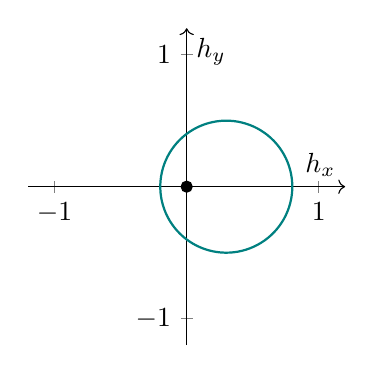
\begin{tikzpicture}
			\begin{axis}[
				axis equal image,
				axis lines=middle,
				axis line style={->},
				xtick={-1,1}, ytick={-1,1},
				xmin=-1.2, xmax=1.2,
				ymin=-1.2, ymax=1.2,
				xlabel=$h_x$, ylabel=$h_y$,
				width=6.5cm,
				]
				\addplot+[mark options={black}] coordinates {(0,0)};
				\addplot [
				samples=100, domain=0:2*pi, color=teal, thick,
				] ( {.5*cos(deg(x)) + 0.3}, {.5*sin(deg(x))} );
			\end{axis}
		\end{tikzpicture}
		\caption{$v=0.3$, $w=0.5$}
	\end{subfigure}
	\caption{Contours in Hamiltonian space for (a) trivial, (b) conducting and (c) topological phases.}
	\label{fig:phases}
\end{figure}

Now that we have a simple setup, it's time to analyse the physics. Concretely, the momentum space Hamiltonian is given by
\begin{align*}
	H(k) &= \h(k)\cdot\bm{\upsigma} = \big(v + w\cos(k)\big)\sigma_x + w\sin(k)\sigma_y = \begin{pmatrix}
		0 & v + w\e^{-ik} \\
		v + w\e^{ik} & 0
	\end{pmatrix}.
\end{align*}
We can set up a Fourier transform to real space by rewriting this suggestively in terms of the unit cell index $n$:
\[
	H(k) = \e^{-ik(n-n)}\begin{pmatrix}
		0 & v \\
		v & 0
	\end{pmatrix} + \e^{-ik\big((n+1)-n\big)}\begin{pmatrix}
		0 & w \\
		0 & 0
	\end{pmatrix} + \e^{-ik\big(n-(n+1)\big)}\begin{pmatrix}
		0 & 0 \\
		w & 0
	\end{pmatrix}
\]
{\color{red} I need to work out the details of this Fourier transform later, my calculations aren't working out. Transforming from a periodic Brillouin zone to (discrete or infinite) real space is breaking my brain. I imagine it needs to look something like this (where $M_{0/\pm1}$ are the three matrices above):
\begin{align*}
	\hat{H} &= \int_B H(k) \ket{k}\bra{k} \\
		&= \int_{-\pi}^{\pi}\frac{\dd{k}}{2\pi} \left(\sum_{a\in\{0,\pm1\}}\e^{-ika}M_a\right) \left(\sum_{n}\e^{-ikn}\ket{n}\right) \left(\sum_{n'}\bra{n'}\e^{ikn'}\right) \\
		&= \sum_{a,n,n'}\left(\int_{-\pi}^{\pi}\frac{\dd{k}}{2\pi}\e^{-ik(a+n-n')}\right)M_a\ket{n}\bra{n'} \\
		&= \sum_{a,n,n'}\delta_{n+a,n'}M_a\ket{n}\bra{n'} \\
		&= \sum_{a,n}M_a\ket{n}\bra{n+a}
\end{align*}
But I don't fully understand the first step, the sign of $a$ is wrong and normalization is broken. Maybe it's easier to discretize first and do a DFT?}

{\color{blue}
\begin{itemize}
	\item It follows [how exactly?] that we can write the Hamiltonian in a unit cell basis as
	\[
		\hat{H} = \sum_{n=-\infty}^{\infty}\left[\ket{n}\bra{n}\otimes\begin{pmatrix}
			0 & v \\
			v & 0
		\end{pmatrix} + \left(\ket{n+1}\bra{n}\otimes\begin{pmatrix}
			0 & w \\
			0 & 0
		\end{pmatrix} + {\rm h.c.}\right)\right]
	\]
	
	\item Mention tight binding somewhere around this point
\end{itemize}
}

It's clear that we have a term parametrized by $v$ which acts within the unit cells, and terms depending on $w$ which act between neighbouring unit cells. To further elucidate the structure of these interactions, we go to a finite chain of length $N$; the Hamiltonian then becomes
\[
	\hat{H} = \sum_{n=0}^{N}\ket{n}\bra{n}\otimes\begin{pmatrix}
		0 & v \\
		v & 0
	\end{pmatrix} + \sum_{n=0}^{N-1}\left(\ket{n+1}\bra{n}\otimes\begin{pmatrix}
		0 & w \\
		0 & 0
	\end{pmatrix} + {\rm h.c.}\right),
\]
where we've introduced open boundary conditions on the ends of the chain, allowing us to study the boundary behaviour in a moment. We can then expand the tensor product in order to cast the Hamiltonian into a full $2N\times 2N$ matrix:
\[
	\hat{H} = \begin{pNiceMatrix}
		\Block[borders={bottom,right,tikz=dashed}]{2-2}{}
					 0 & v & \Block[borders={bottom,right,tikz=dashed}]{2-2}{}
							 0 & 0 & \Block{4-4}{0} &        &   & \\
					 v & 0 & w & 0 &                &        &   & \\
		\Block[borders={bottom,right,tikz=dashed}]{2-2}{}
					 0 & w & 0 & v &                &        &   & \\
					 0 & 0 & v & 0 &                &        &   & \\
		\Block{4-4}{0} &   &   &   &                & \Ddots & 0 & 0 \\
					   &   &   &   & \Ddots         &        & w & 0 \\
					   &   &   &   &              0 & w      & 0 & v \\
					   &   &   &   &              0 & 0      & v & 0
	\end{pNiceMatrix}.
\]
A clear interpretation of this system presents itself to us immediately: it describes a chain of $2N$ sites, with alternating hopping amplitudes $v$ and $w$ between neighbouring sites. The unit cells now consist of two of these sites, and $v$ and $w$ are referred to as the \emph{intra-cell} and \emph{inter-cell} hoppings, respectively. In particular, the gapless phase $v=w$ corresponds to a chain where all hoppings are equal; intuitively, this allows electrons to move around freely along the chain, whereas they are confined around the stronger hoppings in the insulating cases.

The division of our unit cells into two sites allows us to distinguish two \emph{sublattices} of the crystal, which we label $A$ and $B$. We then simplify our notation by labelling quantum states according to the sublattice that they are localized to:
\[
	\ket{n,A} \equiv \ket{n}\otimes\begin{pmatrix}
		1 \\ 0
	\end{pmatrix},\quad \ket{n,B} \equiv \ket{n}\otimes\begin{pmatrix}
		0 \\ 1
	\end{pmatrix}.
\]
In this notation, our Hamiltonian becomes
\begin{equation}\label{eq:ssh-sublattice}
	\hat{H} = \left(\sum_{n=0}^{N}v\ket{n,B}\bra{n,A} + \sum_{n=0}^{N-1}w\ket{n+1,A}\bra{n,B}\right) + {\rm h.c.}
\end{equation}

The picture of alternating hoppings that we have arrived at is precisely the original motivation for this model: it was first introduced in 1979 by Wu-Pei Su, John Robert Schrieffer, and Alan J. Heeger in order to study the properties of polyacetylene (Figure \ref{fig:polyacetylene}), a polymer chain which features alternating single and double covalent bonds \cites{SSH_model}{SSH_model2}.
\begin{figure}[htb!]
	\centering
	\includegraphics[width=.8\linewidth]{Images/polyacetylene} %TODO svg
	\caption{Structural diagram of polyacetylene. Electrons are transported more readily along the double bonds, which is modelled using a larger hopping potential.}
	\label{fig:polyacetylene}
\end{figure}
This material displays unexpectedly high conductivity when doped with halogen impurities, and the SSH model helps explain this behaviour.

To understand how this conductive behaviour comes about, we need to examine the differences between the trivial and the conductive phase somewhat more closely. At a first glance, the two phases appear to be identical: if we choose the unit cell in polyacetylene in such a way that the stronger double bond represents the intra-cell hopping $v$, then we are in the trivial phase $v>w$, and if we center the unit cell around a single bond, we have $v<w$ and the phase is topological. In either case we expect valence electrons to remain localized around the double bonds, leading to the same insulating bulk behaviour.\footnote{
	The attentive reader might wonder why the conductive $v=w$ phase does not occur naturally in this system. This is a result of the so-called Peierls transition: in a nutshell, introducing a band gap locally lowers the energy of the (filled) valence band and raises that of the (empty) conduction band. This makes it energetically favourable for atoms in the chain to pair up, in a process referred to as dimerisation.}

The difference between the two phases only becomes apparent when we look at the endpoints of the chain. For example, the leftmost atom is not subject to any inter-cell hopping, and it is only connected to the other atom in its unit cell. In the trivial case this connection is strong and the two atoms share their valence electrons. On the other hand, in the topological phase the second atom from the left prefers to share electrons with its right-hand neighbour, and the leftmost atom becomes isolated. In the limit where $v$ goes to zero, this isolation becomes complete and the edge sites carry zero-energy eigenstates: in this case only the second term in the Hamiltonian (\ref{eq:ssh-sublattice}) survives, and we have
\begin{align*}
	\hat{H}\ket{1,A} = \hat{H}\ket{N,B} = 0.
\end{align*}
Even for non-zero $v$ the topological phase has edge modes, which can be shown to become highly localized and approach zero energy in the $N\to\infty$ limit. The exact mechanics of this are beyond the scope of this review; the interested reader is referred to e.g.\ \cite{Asboth_topo-course}. The salient point is that the boundary modes of the chain are gapless: their energy eigenvalues have a degeneracy at the Fermi level $\varepsilon_F = 0$.
%TODO picture?

Something remarkable has happened: we have started from a topological description of a gapped bulk phase, and the resulting physical effects appear as gapless edge modes on the boundary of the material. As we will see, this is a fairly\footnote{
	This is not a completely general statement: topological phases with gapped edge modes have been shown to be theoretically feasible \cite{Freedman_gapped-edge}. For our purposes, it will do to restrict our attention to the gapless edge modes.}
general feature of topological phases of matter, called the \emph{bulk-boundary correspondence}. We can think of it as being a result of the inability to go continuously from a topological gapped phase to a trivial one in real space; in particular, the outside boundary of an idealised material connects to the vacuum, which is also considered a trivial gapped phase.

{\color{blue}
\begin{itemize}
	\item Discuss physics of polyacetylene (solitons on trivial/topological interface) and experimental observations of solitons + berry phase \cites{Meier_SSH-soliton}{Atala_SSH-Zak}
	
	\item We can now physically interpret the meaning of setting $h_z = 0$: it ensures that hopping only occurs between the two sublattices $A$ and $B$, and not within them (i.e.\ there are only off-diagonal elements in the internal degrees of freedom). If we define the sublattice projection operators
	\[
		\hat{P}_A = \mathbb{I} \otimes \begin{pmatrix}
			1 & 0 \\ 0 & 0
		\end{pmatrix},\quad \hat{P}_B = \mathbb{I} \otimes \begin{pmatrix}
			0 & 0 \\ 0 & 1
		\end{pmatrix}
	\]
	then the Hamiltonian obeys
	\[
		\hat{P}_A\hat{H}\hat{P}_A = \hat{P}_B\hat{H}\hat{P}_B = 0
	\]
	and so since $\hat{P}_A + \hat{P}_B$ is the identity we have
	\begin{align*}
		\hat{H} &= (\hat{P}_A + \hat{P}_B)\hat{H}(\hat{P}_A + \hat{P}_B) \\
			&= \hat{P}_A\hat{H}\hat{P}_B + \hat{P}_B\hat{H}\hat{P}_A \\
			&= (\hat{P}_A - \hat{P}_B)\hat{H}(\hat{P}_B - \hat{P}_A) \\
			&\equiv -\hat{\Gamma}\hat{H}\hat{\Gamma}
	\end{align*}
	with $\hat{\Gamma}\equiv\hat{P}_A - \hat{P}_B$ having the property that $\hat{\Gamma} = \hat{\Gamma}^{-1} = \hat{\Gamma}\dagger$; this is called sublattice symmetry and it also applies to the momentum space Hamiltonian $H(k)$.
	
	\item An immediate consequence of our setup is that the trivial and topological phase become adiabatically connected if we allow for sublattice symmetry breaking ($h_z \neq 0$).
	
	\item Talk more about $\Z$ invariant (next nearest neighbour hopping etc.)
\end{itemize}
}

\subsection{The Kitaev chain}

{\color{blue}
\begin{itemize}
	\item Introduce Majorana modes
	
	\item Talk about superconductivity
	
	\item Discuss $\Z_2$ invariant vs.\ $\Z$ for SSH topologically
\end{itemize}
}


\section{Two-dimensional models}

\subsection{Quantum Hall effect}

\subsection{The Kane--Mele model}


\markedsection{Symmetry classes}{Classification of symmetries}
	
\chapter{Weyl semimetals}\label{chap:WSM}

In recent years, interest in topological materials has expanded beyond the purely gapped phases in insulators and superconductors, into the realm of metals and other related gapless phases. Some of the topological conductors that are of the greatest interest are called Weyl semimetals, which form the focus of the rest of the present work.

Weyl semimetals are materials that host gapless modes only at very specific momenta in the Brillouin zone. They have a myriad of properties that make them worthy subjects of study, not only from a theoretical perspective but also in potential experimental and engineering applications. Practically, Weyl semimetals have exotic transport properties such as a resistance which is highly sensitive to the application of a magnetic field, opening up countless possibilities for electronic applications. 

Experimentally, Weyl semimetals may comprise the first platform in which the chiral fermions described by Herman Weyl in 1929 can be studied in the wild, %TODO ref
in the form of bulk quasiparticle excitations---despite their mathematical simplicity, Weyl fermions do not appear to exist as fundamental particles in nature. %TODO wording

This aspect of Weyl semimetals is also of theoretical interest, since their fermionic modes may be altered in different ways beyond the simple description originally given by Weyl. Additionally, the topology of Weyl semimetals is intrinsically rich and generalises many aspects of insulator topology. It is this latter topological point of view which is the main focus of this chapter; the interested reader is referred to Refs.~\red{[Armitage]} and \red{[Hosur]} for more complete physically-minded overviews. %TODO refs

This chapter does not contain any new results; instead, its purpose is to provide the necessary context for the results contained in Chapter~\ref{chap:non-orientable}. We begin by introducing the most important physical aspects of Weyl semimetals in Section~\ref{sec:semimetal-physics}, with a focus on the features that are of topological relevance. Section~\ref{sec:semimetal-topology} then dives deeper into the underlying topology, introducing many of the relevant mathematical concepts at a fairly elementary level.

\section{Physical aspects}\label{sec:semimetal-physics}

The concept of Weyl semimetals arises naturally when studying how different energy bands relate to each other in three-dimensional solids. Whereas one and two-dimensional materials are generally gapped unless additional symmetries force the bands to touch, the situation is different in three dimensions. In this context, so-called \emph{accidental band crossings} are expected based on geometric arguments \red{[Herring, 1937]}. %TODO Herring 1937

Accidental crossings can be understood by studying the interplay between any two of the energy bands. In most physically relevant scenarios these will be the valence and conduction band, since these determine the conductive properties of a material. Recall that the generic Hermitian two-band Hamiltonian can be written as
\begin{equation*}
	\Hc(\k) = h_0(\k)\Id + \h(\k)\cdot\bm{\upsigma},
\end{equation*}
where $\k$ lives in the three-dimensional Brillouin torus $\T^3$ in this case. The eigenvalues of this Hamiltonian are
\begin{equation*}
	E(\k) = h_0(\k) \pm \abs{\h(\k)} = h_0(\k) \pm \sqrt{h_1^2(\k) + h_2^2(\k) + h_3^2(\k)},
\end{equation*}
so that the gap between the two bands closes exactly when $\h(\k) = 0$. That is, band crossings occur at the simultaneous zeroes of three functions $h_i$ for $i\in\set{1,2,3}$, all depending on three momentum degrees of freedom. Such a system of three equations with three parameters generically has point-like solutions: the zeroes of each individual $h_i$ normally form a surface in $\T^3$, two such surfaces intersect in a set of curves, and the third surface intersects these curves in a set of points. This means that two bands in a three-dimensional system generically have point-like intersections where the gap closes, given that the bands are close enough together (i.e.\ the functions $h_i$ each have zeroes to begin with). %TODO repetitions
These band crossings are called accidental because they are not enforced by any symmetry of the system, but as we will review shortly, they are actually topologically robust and cannot be gapped out by small perturbations.

\subsection{Weyl points}
Near a band intersection at $\k=\k_w$, the Hamiltonian can be linearized: writing $\delta\k := \k - \k_w$, it can be expanded as
\begin{equation}\label{eq:linearized-Hamiltonian}
	\Hc(\delta\k) = h_0(\k_w)\Id + \vb{v}_0\cdot\delta\k\Id + \sum_{i=1}^{3}\vb{v}_i\cdot\delta\k \sigma^i + \order{\delta\k^2},
\end{equation} %TODO mention Fermi velocities?
where $(\vb{v}_\mu)_i := \dee_{k^i}h_\mu |_{\k=\k_w}$ records the rate of change of the different components of the Hamiltonian. The spectrum associated with this linear equation looks like two cones which touch at $\k=\k_w$, often collectively called the \emph{Weyl cone}; see Figure~\red{[figure]}. %TODO
%TODO figure
The different components of Equation~\eqref{eq:linearized-Hamiltonian} can all be given an interpretation in terms of this Weyl cone: for example, $h_0(\k_w)$ is the energy at which the bands touch, and it determines how far this crossing is from the Fermi energy $\varepsilon_F=0$. If $h_0$ is sufficiently far from the Fermi level, the Fermi surface expands to connect with those around other band crossings and gains an extensive two-dimensional structure. Normal metallic dispersive behaviour dominates in this case. However, if $h_0$ is close enough to zero, then the Fermi surface around $\k_w$ becomes approximately point-like, and there is a low-energy bulk conductive mode at $\k_w$. In this case the point $\k_w$ is called a \emph{Weyl point} or \emph{Weyl node}. When all of the crossings between the valence and conduction band have this property, the material is referred to as a \emph{Weyl semimetal}.\footnote{
	The term \emph{Weyl metal} is also sometimes used for materials in which the Fermi surface is not point-like due to large $h_0$, but still confined to closed surfaces around the band crossings \cite{Burkov_Weyl-metals}. The topology of such Weyl metals is equivalent to that of their semimetal counterparts, and we will pay them no further mind.}

This nomenclature is derived from the traceless $\vb{v}_i$ term in Equation~\eqref{eq:linearized-Hamiltonian}: it bears resemblance to the simple chiral fermions described by Herman Weyl in 1929 \red{[Weyl, 1929]}, %TODO Weyl 1929 %it bears resemblance to the Hamiltonians describing individual Weyl fermions
\begin{equation*}
	H_\pm = \mp c\vb{p}\cdot\bm{\upsigma},
\end{equation*}
where the speed of light $c$ is replaced by the smaller effective velocities $\vb{v}_i$ in different directions. In a Weyl semimetal, the aforementioned low-energy modes have similar dispersive properties to Weyl fermions. This is one of the reasons Weyl semimetals are a desirable object of study, especially since---despite their mathematical simplicity---Weyl fermions have not been observed as fundamental particles in nature.

One particularly interesting feature of Weyl fermions is that they have a non-zero chirality associated with them, which leads to certain non-conserved charges upon quantisation---this is known as the chiral anomaly. It turns out that a similar truth holds for the band crossings described by Equation~\eqref{eq:linearized-Hamiltonian}. They feature an intrinsic chirality $\chi$, which can be calculated in generic cases by collecting the velocities $\vb{v}_i$ into a $3\times 3$ matrix $V_i^j := (\vb{v}_i)_j$ and computing the sign of its determinant:
\begin{equation}\label{eq:determinant_chirality}
	\chi = \sign{|V_i^j|},
\end{equation} 
giving a chirality of $\chi=\pm1$. In special cases where the band crossing is non-linear, the chirality may take on other integer values; this is captured more generally using a Berry curvature integral on a two-dimensional sphere surrounding the Weyl point. In this light, Weyl points can be viewed as sources or sinks of the Berry field, with a quantized integer charge. This charge is topological in nature, which is exactly why Weyl points are robust to perturbations. The implications of this topological perspective will be explored in greater detail in Section~\ref{sec:semimetal-topology}.

A final feature of Equation~\eqref{eq:linearized-Hamiltonian} that bears mentioning is the inclusion of the $\vb{v}_0$ term. This term can be interpreted in terms of a tilting of the associated Weyl cone. For small $\vb{v}_0$, the Fermi surface of a Weyl point remains point-like, and the dispersive properties of the virtual Weyl fermion aren't greatly affected. However, for large enough $\vb{v}_0$, the Weyl cone may begin to intersect the Fermi level, causing electron and hole pockets to form on either side of the Weyl point; see Figure~\ref{fig:Weyl-cone-tilt}.
\begin{figure}[htb!]
	\centering
	\includegraphics[width=.7\linewidth]{Images/Weyl-cone-tilt}
	\caption{Figure from Ref.~\cite{Soluyanov_Type-II}. Left: Weyl cone in a normal (type I) Weyl semimetal. Right: ``Overtilted'' Weyl cone in a type II Weyl semimetal. Electron and hole pockets are outlined in red and blue, respectively.}
	\label{fig:Weyl-cone-tilt}
\end{figure}
This tipping of the Weyl cone induces significantly altered dispersion, leading to different electronic properties. Such materials are categorised separately as so-called \emph{type II} Weyl semimetals. %TODO type II NODES; also mention type I
This distinction is purely physical, however; the different types of Weyl semimetals cannot be distinguished topologically.

\subsection{Global features}

One important restriction on Weyl semimetals is that the total chirality of all Weyl points in the Brillouin zone must sum to zero---that is, for every source of the Berry field (Weyl point with $\chi>0$) there must also be a sink ($\chi<0$), and vice versa. This result is known as the Nielsen--Ninomiya theorem, after Holger Bech Nielsen and Masao Ninomiya who proved it in a more general context in 1981 \cite{NielsenNinomiya_I,NielsenNinomiya_II}. We will explore the topological nature of this theorem in more detail in Section~\ref{sec:semimetal-topology}. Physically, this charge cancellation is related to the aforementioned chiral anomaly: electric charge is locally non-conserved near a Weyl point under the application of electric and magnetic fields, and this effect must be cancelled by a Weyl point of the opposite chirality. More details on the chiral anomaly in Weyl semimetals are reviewed in Ref.~\cite{Hosur_WSM-transport}.

The Nielsen--Ninomiya theorem is an indication that Weyl points must communicate with their opposite-chirality counterparts in some way to allow transport of charge. This connection manifests itself on the surface of a Weyl semimetal: there, gapless states called \emph{Fermi arcs} appear in the form of curves connecting the projections of oppositely-charged Weyl points; see Figure~\ref{fig:WSM_bulk+arc}.
\begin{figure}[htb!]
	\centering
	\includegraphics[width=.5\linewidth]{Images/WSM_bulk+arc}
	\caption{Figure by Alan Stonebraker. The 3D bulk Brillouin zone is shown of a Weyl semimetal with two Weyl points of negative and positive chirality, depicted as a sink and a source of the Berry field respectively. A 2D surface Brillouin zone is also depicted in grey at the top, featuring the projection of the two Weyl nodes connected by a Fermi arc of gapless states.}
	\label{fig:WSM_bulk+arc}
\end{figure}
Fermi arcs serve as important experimental signatures of Weyl semimetals, and they have been observed in both electronic and artificial crystals since 2015  \cite{Weng_WSM-candidates,Huang_WSM-candidates,Lv_WSM-TaAs,Xu_WSM-experiment,Belopolski_minimal-WSM,Liu_photonic-Chern-vector}; see Figure~\ref{fig:TaAs_experiment}.
\begin{figure}[htb!]
	\centering
	\includegraphics[width=.6\linewidth]{Images/TaAs_experiment}
	\caption{Figures from Ref.~\cite{Xu_WSM-experiment}. Experimental bulk (orange) and surface (green) Fermi surfaces, obtained through angle-resolved photoemission spectroscopy (ARPES). Bottom left: Two Weyl points appearing close together in the bulk. Top left: Fermi arcs are shown to terminate on the surface Brillouin zone above these Weyl points. Right: Bulk measurements are overlaid on the surface measurements at matching $k_x$ and $k_y$ values, showing good agreement between the position of the Weyl nodes and the tail ends of the Fermi arcs. In this case the two distinct Fermi arcs appear because there are two separate sets of Weyl nodes with the same $k_x$ and $k_y$ coordinates.}
	\label{fig:TaAs_experiment}
\end{figure}


\subsection{Semimetals with symmetries}

Thus far, we have discussed Weyl semimetals without assuming any additional symmetry constraints. However, real crystalline solids often naturally possess symmetries beyond simple translational symmetry. Two such symmetries which are especially relevant to the discussion of Weyl semimetals are time-reversal symmetry and inversion symmetry.

Inversion symmetry is a natural property of many real-space lattices: it implies that there is an inversion centre $\vb{x}_0$ in the unit cell around which the lattice is symmetric as $\vb{x}\leftrightarrow\vb{x}_0-\vb{x}$. In momentum space, this symmetry acts on the Hamiltonian as
\begin{equation}\label{eq:inversion-symmetry}
	\Hc(\k) = U\Hc(-\k)U\herm,
\end{equation}
where $U$ is some unitary transformation. In particular, this implies that a Weyl point at $\k=\k_w$ has a partner at $\k=-\k_w$ with the opposite chirality. Take for example the case of $U=\Id$ and a Weyl point with the simple linearized Hamiltonian 
\begin{equation*}
	\Hc(\delta\k) = \sum_{i,j}V_i^j\delta k_j \sigma^i.
\end{equation*}
This point has chirality $\chi = \sign\abs{V_i^j}$, and Equation~\eqref{eq:inversion-symmetry} implies that
\begin{equation*}
	\Hc(-\delta\k) = \sum_{i,j}(V')_i^j(-\delta k_j)\sigma^i = \Hc(\delta\k),
\end{equation*}
meaning there is a Weyl point at $\k=-\k_w$ with chirality $\chi' = \sign\abs{(V')_i^j} = \sign\abs{-V_i^j} = -\chi$. This reversal of chirality means Nielsen--Ninomiya is automatically satisfied under inversion symmetry. As a result, the minimum number of Weyl points in such a system is two; a Weyl point may be connected to its own symmetric partner via surface Fermi arcs.

Time-reversal symmetry has a similar action in momentum space, since momentum has a time component. It differs in the sense that time-reversal is an anti-unitary symmetry, meaning it also induces complex conjugation on the Hamiltonian:
\begin{equation*}
	\Hc(\k) = U\Hc^*(-\k)U\herm.
\end{equation*}
This complex conjugation changes the sign of the $\sigma^2$ term in the Hamiltonian; for Weyl points, this changes the sign of $\vb{v}_2$, inducing a sign change in the determinant of $V_i^j$. This cancels the sign change discussed above, meaning a Weyl point at $\k=\k_w$ always comes with a symmetric partner of \emph{equal} chirality at $\k=-\k_w$. Such a pair of equal-chirality points is sometimes referred to as a \emph{Kramers pair}. The presence of Kramers pairs means the minimum number of Weyl points in a time-reversal invariant Weyl semimetal is four: following Nielsen--Ninomiya, a pair of $\chi = +1$ points must always be accompanied by a pair of $\chi=-1$ points and vice versa.

The fact that the chirality of Weyl points is reflected in different ways under inversion and time-reversal symmetry immediately implies that a Weyl semimetal cannot satisfy both symmetries at once: if a Weyl point has a non-zero chirality $\chi$, then inversion implies its partner has chirality $-\chi$, while time-reversal implies it should have chirality $\chi$. Physically, this is because the combination of inversion and time-reversal induces a spin degeneracy in the band structure, making modes of opposite chiralities coincide. This is in close analogy to the way in which a Dirac fermion combines two Weyl fermions of opposite chirality into a single description; this is precisely why band touching points of this nature are called \emph{Dirac cones}, and systems featuring them are referred to as \emph{Dirac semimetals}. Because of the lack of non-zero chiralities, such materials are topologically less rich than their Weyl counterparts, and we will not expand on them further.

All in all, a candidate Weyl semimetallic material must break either inversion or time-reversal symmetry. Of the two, breaking time-reversal symmetry is conceptually simpler in theory: the minimum amount of Weyl points is lower, and the symmetry is straightforwardly broken in the presence of a magnetic field. However, in practice the experimental detection of Fermi arcs and other spectral features relies on angle-resolved photoemission spectroscopy (ARPES), which is sensitive to magnetic fields. This is why to date, all experimentally confirmed electronic Weyl semimetals have preserved time-reversal symmetry and broken inversion symmetry instead  \cite{Weng_WSM-candidates,Huang_WSM-candidates,Lv_WSM-TaAs,Xu_WSM-experiment,Belopolski_minimal-WSM}.


\section{Topological description}\label{sec:semimetal-topology}

In all the systems studied in Chapter~\ref{chap:topo-states}, the underlying approach to topological classification has been to study which band structures cannot be deformed into each other without closing the band gap anywhere in the Brillouin zone. Weyl semimetals already feature band crossings in the bulk to begin with, meaning this approach needs to be modified. The basic idea involves fixing a number of gapless points in place first, and then studying what gapped topologies are admitted on the rest of the Brillouin zone outside of these points. There are many intricacies to this idea, some of which we attempt to review pedagogically in this section.

Though most of the experimental candidates for Weyl semimetals feature either inversion or time-reversal symmetry, the conceptual topology framework is simplest in the absence of any symmetries beyond lattice translation. The majority of this section is written with this context in mind. Most of the concepts here are borrowed from two superb (if fairly technical) works by Vargese Mathai and Guo Chuan Thiang \cite{Mathai_math-review,Mathai_math-paper}.

Only in the final part of this section will we return to time reversal symmetric systems, and review how the inclusion of this symmetry alters the topological description. This provides important context to our treatment of other symmetries in Chapter~\ref{chap:non-orientable}.

The topological arguments in this section rely heavily on the concepts of cohomology and homology. Where possible, an attempt is made to explain the relevant ideas ``just enough'' in their proper physical context so that the main flow of the text may be followed without the relevant mathematical background. Readers seeking a somewhat more fundamental understanding are invited to refer to Appendix~\ref{chap:homology} as needed.

\subsection{3D Chern insulators}

To get a good intuition for the topological description of Weyl semimetals, it is useful to first consider a fully insulating material with similar properties. Suppose we have a three-dimensional material that is not subject to any additional symmetries. Such a material is called a 3D Chern insulator \cite{Vanderbilt_2018,Liu_photonic-Chern-vector,Devescovi_3D-Chern}, in analogy to the 2D Chern insulator studied in Section~\ref{sec:Chern}. This system is not a semimetal, but it provides the relevant topological backdrop: Weyl semimetals can be obtained by letting the bands touch in a 3D Chern insulator. As we will discuss shortly, this allows them to act as transitional phases between different insulating topological states.

From the Atland--Zirnbauer classification in Table~\red{[reference]}, %TODO ref. to tenfold way table
one might expect such a 3D type A system to be topologically trivial. However, as seen before in Equation~\red{[reference] (and perhaps also in 3D BHZ/Kane--Mele if I discuss this in ch. 2)}, %TODO ref. to weak topology equation
the full topological classification of materials depends not only on the top-dimensional topology, but also on that borrowed from lower-dimensional subspaces. In the case of a 3D Chern insulator, this topology arises on two-dimensional slices of the Brillouin zone; an example of such a slice is highlighted in Figure~\ref{fig:3D_Chern_insulator}.
\begin{figure}[htb!]
	\centering
	\includegraphics[width=.5\linewidth]{Images/3D_Chern_insulator}
	\caption{Figure adapted from Ref.~\cite{Mathai_math-review}. The three-dimensional Brillouin torus $\T^3$ of a Chern insulator is shown, with a two-dimensional slice $\T_{yz}^2$ indicated in blue. A projection onto a surface Brillouin zone in the $xy$-direction is also shown, with an example Fermi loop of gapless states in red. In this example, the slice $\T_{yz}^2$ has a Chern number of $C_{x} = 1$. Hence, its projection onto the surface is a 1D loop (blue line) that features one chiral band crossing.}
	\label{fig:3D_Chern_insulator}
\end{figure}

There are three topologically distinct ways to slice up the three-torus, all perpendicular to one of the three coordinate directions.\footnote{
	Other 2D slices exist, such as those going diagonally across, but these can all be considered linear combinations of the three ``orthogonal'' slices. To be precise, the different classes of 2D subspaces of $\T^3$ form the second homology group $H_2(\T^3)\cong\Z^3$, and this group is \emph{generated} by the orthogonal slices.}
These slices have the topology of a two-torus $\T^2$, and a Chern number can be obtained by integrating the Berry curvature $\Fc$ of the system over them: for example, perpendicular to the $x$ direction there is a Chern number\footnote{
	Note that it does not matter where along the Brillouin zone the $yz$-slice $\T_{yz}^2$ is taken: the Chern number is an integer, while the system is continuous. This means the $x$ coordinate can be changed continuously without changing the resulting Chern number.}
\begin{equation*}
	C_{x} = \frac{1}{2\pi}\int_{\T_{yz}^2}\!\Fc.
\end{equation*}
This results in a classification by three distinct Chern numbers $C_x$, $C_y$ and $C_z$, which are commonly arranged in a so-called \emph{Chern vector}
\[
	\vb{C} = \begin{pmatrix}
		C_x \\ C_y \\ C_z
	\end{pmatrix} \in \Z^3.
\]

Importantly, these three Chern numbers are all induced by a single two-form $\Fc$. In this sense, there is an exact correspondence between topologically distinct Berry curvatures $\Fc$ and Chern vectors $\vb{C}\in\Z^3$. This is precisely what motivates the use of cohomology for classification: just like in the 2D Chern insulator, the two-form $\Fc$ can be considered to represent a class in the second cohomology group,\footnote{
	As explained in Appendix \ref{chap:homology}, $\Fc$ more properly represents a class in the real-valued \emph{de Rham cohomology} group $H_{\rm dR}^2(\T^3)\cong\R^3$. The analogy is strong enough to be considered direct here, but de Rham cohomology is too plain to encode features such as $\Z_2$ invariants. This is why we make use of the richer integer-valued cohomology theory.} %TODO perhaps move to ch.2
\begin{equation}\label{eq:2nd-cohom-t3}
	[\Fc]\in H^2(\T^3)\cong\Z^3. 
\end{equation}
As a result, this group precisely classifies the distinct topological phases of the system.\footnote{
	More fundamentally, a complex vector bundle called the \emph{valence bundle} can be associated to a gapped Hamiltonian, and the second cohomology group classifies the different complex vector bundles over a manifold.} %TODO maybe move this to ch.2

\subsubsection{Boundary states}

Before moving on to a system with Weyl points, it will be instructive to study the gapless modes that arise on the surface of a 3D Chern insulator with non-zero Chern vector. Figure~\ref{fig:3D_Chern_insulator} illustrates the case where $\vb{C} = (1,0,0)\tran$. In this case, $\T_{yz}^2$ is the only orthogonal slice with a non-zero Chern number, and as such the material lattice can be thought of as a stack of 2D Chern insulators spanning the $y$ and $z$ directions, stacked together in the $x$ direction. $\T_{yz}^2$ can effectively be considered the Brillouin zone of such a 2D Chern insulator.

Recall from our discussion in Section \ref{sec:Chern} that a 2D Chern insulator with a Chern number of 1 has a single chiral edge mode, which manifests as a gapless state on the one-dimensional surface Brillouin zone. This logic can be translated to the the three-dimensional case, where such slices are stacked in the $x$ direction. Suppose there is a projection $\pi$ along the $z$ direction, onto a two-dimensional surface Brillouin zone $\ext{\T}_{xy}^2$. Then the two-dimensional slices $\T_{yz}^2$ project down to a one-dimensional loop $\pi(\T_{yz}^2)\cong S^1$ containing a single point-like gapless state. As the $\T_{yz}^2$ slice is moved around in the $x$ direction, this band crossing point moves continuously along the $y$ direction, by continuity of the Hamiltonian. It follows that the full two-dimensional surface Brillouin zone must contain a loop of gapless states going across the $x$ direction, as depicted in the figure. This loop is called a \emph{Fermi loop}, in analogy with the Fermi arcs in a Weyl semimetal . Moreover, the chirality of the edge modes can be used to assign a consistent orientation to this loop. %TODO note about linked loops, extra topology etc? Might be unnecessary

Fermi loops admit a natural topological description in terms of homology. Being oriented loops, they precisely represent a class in the first homology group $H_1(\ext{\T}^2)$ of the surface Brillouin zone. Furthermore, it is possible to define an oriented \emph{Dirac loop} $\ell$ in the bulk Brillouin zone in such a way that its projection $\pi(\ell)$ onto the surface in any direction is exactly the Fermi loop. This loop $\ell$ is not a gapless feature,\footnote{ %TODO wording: "gapless feature" not necessarily standard, explain more
	Dirac loops do still admit a physical interpretation: they represent points at which the Berry connection $\Ac$ has a gauge singularity. Such singularities depend on the choice of gauge, meaning the loop can be moved around by gauge transformations; however, this does not change their topology. The same goes for the Dirac strings that will be discussed in a moment.}
but it is rather interesting topologically: it represents a first homology class in the bulk Brillouin zone,
\[
	[\ell]\in H_1(\T^3)\cong\Z^3.
\]

It is not a coincidence that this first homology group is isomorphic to the second cohomology group $H^2(\T^3)$ from Equation~\eqref{eq:2nd-cohom-t3}. This equivalence is a result of \emph{Poincar\'e duality}, which is the statement that for any closed oriented $d$-dimensional manifold $M$, the isomorphism
\[
	H_n(M) \cong H^{d-n}(M)
\]
holds for any integer $n$. In the present case, this duality can be stated intuitively in terms of Chern numbers, which count the number of signed intersections of the Dirac loop with the different two-dimensional slices of the Brillouin zone.\footnote{
	In general, it is possible that a single Dirac loop ``folds back on itself'' and intersects such a slice more than once. However, any additional intersections introduced in this way always come in oppositely-oriented pairs, leaving the topology unchanged.}
This duality can be summarised schematically as follows:
\begin{equation}\label{eq:duality-scheme}
	H^2(\T^3) \ni [\Fc] \overset{\rm integration}{\iff}
	\vb{C} \overset{\rm intersections}{\iff} [\ell] \in H_1(\T^3).
\end{equation}
This Poincar\'e duality ensures that the classifications in terms of first homology and second cohomology are completely equivalent in this case. Importantly, however, Poincar\'e duality depends on orientability, and it will not hold when we consider non-orientable Brillouin zones in the next chapter. As such, the question of which group provides the right classification of such a system will be key. For the moment, we turn our attention to the topology of Weyl points in the simpler orientable setting.


\subsection{Topology with Weyl points}\label{sec:Weyl-point-topology}

Consider a Weyl semimetal with a set of $k$ Weyl points
\[
	W \equiv \set{w_1,w_2,\ldots,w_k}\subset \T^3.
\]
Then the charge of a Weyl point $w_i$ is given by the Chern number
\begin{equation*}
	C_w = \frac{1}{2\pi}\int_{S_w^2}\!\Fc,
\end{equation*}
where $S_w^2$ is a sufficiently small 2-sphere centred at $w$---in particular, it must be small enough to contain no other Weyl points in its interior. Naively, this might lead us to expect that a semimetal phase is classified by the second cohomology group of the collection of all these spheres:
\begin{equation}\label{eq:2nd-cohom-spheres}
	H^2\left(\bigcup_{i=1}^k S_{w_i}^2\right)\cong \bigoplus_{i=1}^k H^2(S_{w_i}^2) \cong \Z^k.
\end{equation}
However, this classification runs into two problems: it ignores the global cancellation of charge, and it also ignores the additional topology on two-dimensional slices discussed in the previous subsection. Both of these issues are due to the fact that this group only captures the \emph{local} topology near each Weyl point, and they can be addressed by studying how the different Chern numbers on the Brillouin zone must relate to each other \emph{globally}.

The Nielsen--Ninomiya charge cancellation theorem is one such global relation. It is the statement that all the Chern numbers on these 2-spheres must add to zero:
\begin{equation}\label{eq:Nielsen-Ninomiya}
	\sum_{i=1}^{k}C_{w_i} = 0.
\end{equation}
This cancellation can be demonstrated using Stokes' theorem. The argument goes as follows: imagine that the interior of each sphere $S_{w_i}^2$ (i.e.\ a small open 3-ball centred at $w_i$) is removed from $\T^3$. The resulting 3-manifold $X$ looks like a 3-torus with $k$ small ball-shaped holes, and its boundary is given by the collection of spheres:
\[
	\partial X = -\bigcup_{i=1}^k S_{w_i}^2,
\]
where the minus sign induces the correct orientation. Then Stokes' theorem gives
\[
	0 = \frac{1}{2\pi}\int_{\partial X} \dd{\Fc} = -\sum_{i=1}^{k}\frac{1}{2\pi}\int_{S_{w_i}^2}\!\!\Fc = -\sum_{i=1}^{k}C_{w_i},
\]
which is precisely the Nielsen--Ninomiya theorem.

A similar argument can also be applied to study what happens to Chern numbers on two-dimensional slices of the Brillouin zone in this context. This argument is illustrated in Figure~\ref{fig:Weyl-point-Stokes}.
\begin{figure}[htb!]
	\centering
	\includegraphics[width=.5\linewidth]{Images/Weyl-point-Stokes}
	\caption{
		Brillouin torus $\T^3$ of a Weyl semimetal with two oppositely charged Weyl points labelled $+$ and $-$. Three two-dimensional subspaces are indicated in blue: a $yz$-like 2-torus on either side of the $+$ point, and a small 2-sphere surrounding it. Given the proper orientation, the blue spaces form the boundary of a three-dimensional manifold $Y$, shaded in grey here.
		Figure from Ref.~\cite{Mathai_math-review}. \red{[not yet licensed; may need better labelling]}%TODO rights, labelling
	}
	\label{fig:Weyl-point-Stokes}
\end{figure}
Here, two slices $\T_L^2$ and $\T_R^2$ are placed on either side of a Weyl point $w$ with charge $C_w = q$, along with a small sphere $S_w^2$ surrounding it. These spaces then bound a three-dimensional manifold $Y$ as indicated in the figure, given the following orientations:
\[
	\partial Y = \T_R^2 - \T_L^2 - S_w^2.
\]
The same Stokes' theorem argument can then be used to relate the Chern numbers $C_L$ and $C_R$ on the respective slices, yielding
\[
	C_R = C_L + C_w = C_L + q.
\]
That is, the Chern number of a two-dimensional slice increases by $q$ every time it passes over a Weyl point with charge $q$. As a sanity check, it should be noted that this process respects the periodicity of the Brillouin torus: when the slice is passed over the entire torus, charge cancellation ensures that the added Chern number is zero in total.

All in all, the presence of Weyl points allows for a finer collection of Chern numbers to appear in the Brillouin zone, beyond the $\Z^3$ Chern vector of the insulating case. This behaviour can be captured using cohomology. The key idea is that the Berry curvature has a singularity at points where the gap closes.\footnote{
	Note that this singularity is required in order for the Chern number to change suddenly when a slice (i.e.\ the integration domain of $\Fc$) is moved over a Weyl point continuously.}
As such, it can only be integrated over subspaces where the gap never closes, so that the set of Weyl points $W$ needs to be excluded. This means $\Fc$ now lives in the second cohomology group of the Brillouin zone minus $W$:
\begin{equation}\label{eq:2nd-cohom-semimetal}
	[\Fc]\in H^2\big(\T^3\setminus W\big) \cong \Z^3\oplus\Z^{k-1},
\end{equation}
where $k$ again is the number of Weyl points. Put differently, classification of semimetallic phases given a set of Weyl points $W$ essentially amounts to classifying the gapped phases on the punctured torus $\T^3\setminus W$.

Notably, this classification addresses both issues present in the $\Z^k$ classification on 2-spheres in Equation~\eqref{eq:2nd-cohom-spheres}. Firstly, it incorporates 3D Chern insulator topology in the first term, in the form of the $\Z^3$ from Equation~\eqref{eq:2nd-cohom-t3}. Perhaps more subtly, charge cancellation is also incorporated in the form of the reduction by one $\Z$ factor in the second term. This can be understood intuitively: for example, if $k=1$ then the Nielsen--Ninomiya theorem implies that the single Weyl point must have a charge of 0, and so it is not topologically protected. A similar intuition holds for larger $k$, in that the $k$ ``degrees of freedom'' which are afforded to the system by the Weyl point charges are reduced by one under the charge cancellation condition. %TODO wording: 1 equation on k dof
This relation will become more explicit once the Mayer--Vietoris sequence is introduced in Section \ref{sec:Mayer-Vietoris}.

%Notably, there are $k-1$ extra factors of $\Z$ involved in the classification of a Weyl semimetal compared to that of a 3D Chern insulator (cf.\ Equation~\eqref{eq:2nd-cohom-t3}). This contrasts with the $k$ factors found for the collection of spheres in Equation~\eqref{eqeq:2nd-cohom-spheres}. This reduction by one is a natural result of charge cancellation: for example, if $k=1$ then the Nielsen--Ninomiya theorem implies that the single Weyl point must have a charge of 0, and so it is not topologically protected. A similar intuition holds for general $k\in\N$, in that the $k$ additional ``degrees of freedom'' which are afforded to the system by the Weyl point charges are reduced by one under the charge cancellation condition. This relation will become more explicit once the Mayer--Vietoris sequence is introduced in Section \ref{sec:Mayer-Vietoris}.


\subsubsection{Fermi arcs}

The varying Chern numbers over Weyl points help explain how Fermi arcs arise on the surface. As discussed in the case of a 3D Chern insulator, Fermi loops on the surface arise whenever there is a non-zero Chern number in some direction. Similarly, Fermi arcs begin and terminate whenever the presence of a Weyl point causes a change in the Chern number; this is illustrated in Figure~\ref{fig:Fermi-arc-Chern}.
\begin{figure}[htb!]
	\centering
	\includegraphics[width=\linewidth]{Images/Fermi-arc-Chern}
	\caption{
		Two semimetal Brillouin zones are shown with the same configuration of Weyl points, but featuring topologically distinct Fermi arcs (shown in red on the boundary). The distinction is due to different bulk Chern numbers: Fermi arcs appear in regions where the bulk Chern number is non-zero. These Fermi arcs can be considered to be the projection of a Dirac string (shown in red in the bulk).
		Figure from Ref.~\cite{Mathai_math-review}.}
	\label{fig:Fermi-arc-Chern}
\end{figure}

This feature of Weyl semimetals implies they can mediate phase transitions between 3D Chern insulators with different Chern vectors. For example, suppose a pair of Weyl points is created at some point in the Brillouin zone of a trivial insulator ($\vb{C}=0$). These points can then be moved apart in the $z$ direction until they meet again and annihilate at the other end of the torus. In the process, a Fermi arc extends between the projections of the Weyl points on the $xz$ and $yz$-planes, which eventually closes into a Fermi loop. In its final state, the system features a non-zero Chern vector of $\vb{C} = (0,0,1)\tran$.

This process was first observed experimentally in a seminal work by Gui-Geng Liu et al.\ in 2022 \cite{Liu_photonic-Chern-vector}. The authors construct a photonic crystal, which is a type of artificial crystal where the different energy levels are represented by frequencies of light. Under application of a magnetic field, this crystal undergoes a transition between trivial and topological insulating phases, mediated by the creation and annihilation of two Weyl points; see Figure~\ref{fig:Weyl-phase-transition}.
\begin{figure}[htb!]
	\centering
	\includegraphics[width=\linewidth]{Images/Weyl-phase-transition}
	\caption{Figure from Ref.~\cite{Liu_photonic-Chern-vector}, reproduced with permission from Springer Nature.
		Top: measured frequency response (i.e.\ ``band structure'') at increasing magnetic field strength. Yellow regions represent a band gap in the spectrum, indicating insulating phases. The white line represents the calculated frequency of the two Weyl nodes in the system. Bottom: measured response on a surface Brillouin zone, at the frequencies indicated on the white line above. Simulated Fermi arcs and loops are shown in green. A Fermi loop can clearly be seen to form, confirming a phase change to a topological insulator.}
	\label{fig:Weyl-phase-transition}
\end{figure}
This was also the first experimental realisation of a 3D Chern insulator, and of a system featuring a single Fermi arc.

Just as Fermi loops can be considered projections of a bulk Dirac loop, so too can Fermi arcs be considered a projection of a bulk \emph{Dirac string}.\footnote{
	A more or less equivalent concept is referred to as \emph{Euler chain} in Ref.~\cite{Mathai_math-review}, placing the emphasis on topology over physics: ``chain'' here refers the oriented subspaces that homology is founded on.}
Like Dirac loops, these strings can be given an interpretation in terms of homology. The setup is somewhat more subtle in this case: since the Dirac strings have a boundary, they are not loops and as such do not represent homology classes in $H_1(\T^3)$. Instead, they represent classes in the \emph{relative homology group}
\begin{equation}\label{eq:relative-homology}
	H_1\big(\T^3, W\big) \cong \Z^3\oplus\Z^{k-1}
\end{equation}
with respect to the set of Weyl points $W\subset\T^3$. Intuitively, taking the relative homology means that any boundaries lying in the subset $W$ are ignored; for a more precise definition the reader is referred to Ref.~\parencite[\S 2.1]{Hatcher_algebraic-topology}.

This homology picture provides a classification scheme that is exactly dual to the cohomology classification in Equation~\eqref{eq:2nd-cohom-semimetal}; that is, there is an isomorphism
\begin{equation}\label{eq:semimetal-duality}
	H^2\big(\T^3\setminus W\big) \cong H_1\big(\T^3, W\big).
\end{equation}
This is not a direct Poincar\'e duality, but it is nevertheless mathematically rigorous and protected by orientability in the same way.\footnote{
	To be precise, Poincar\'e duality does not hold directly because $\T^3\setminus W$ is not a closed manifold. Instead, for non-compact manifolds $M$ there is a generalized duality $H^n(M)\cong H_{d-n}^{\rm BM}(M)$ where the group on the right is the \emph{Borel--Moore homology}, and this is in turn equivalent to the relative homology in this case. Alternatively, Equation~\eqref{eq:semimetal-duality} can be interpreted as a result of the so-called \emph{Lefschetz duality} $H^n(M)\cong H_{d-n}(M, \partial M)$ for manifolds with a boundary.}
The interpretation in terms of Chern numbers given in Equation~\eqref{eq:duality-scheme} also still holds here, with the Chern vector and Dirac loops replaced with more general Chern numbers and Dirac strings, respectively.


\subsection{The semimetal Mayer--Vietoris sequence}\label{sec:Mayer-Vietoris}

In the previous section, a heuristic Stokes' theorem argument was presented for charge cancellation on Weyl points. This argument can be generalized by moving to a more abstract cohomology setting, where we are not dependent on the integration of forms; this is important because integration will not be well defined once we move to a non-orientable setting. As an added bonus, the abstract description proves to be richer and provide more detailed information on the possible topological phases for a Weyl semimetal.

The idea is that the relation between the global semimetal topology in Equation~\eqref{eq:2nd-cohom-semimetal} and the local charge data in Equation~\eqref{eq:2nd-cohom-spheres} can be understood by considering how cohomology classes are mapped between them. That is, one needs to find and study a homomorphism
\begin{equation*}
	\beta: H^2\big(\T^3\setminus W\big) \to H^2\left(\bigcup_{i=1}^k S_{w_i}^2\right).
\end{equation*}
Such a map arises naturally in the context of the \emph{Mayer--Vietoris sequence} for cohomology.

Mayer--Vietoris sequences are used to study how the homology or cohomology of a topological space relates to that of its subspaces. To be precise, let $X$ be a topological space and let $A,B\subset X$ be two subspaces that cover it (i.e.\ $A\cup B = X$). Then, there is an \emph{exact sequence} of homomorphisms between cohomology groups,
\begin{equation*}
	\cdots \to H^n(X) \to H^n(A)\oplus H^n(B) \to H^n(A\cup B) \to H^{n+1}(X) \to \cdots,
\end{equation*}
which continues indefinitely %TODO not really indefinitely
in both directions. Exactness means that the image of each map in the sequence is exactly equal to the kernel of the next. %TODO introduce notation
In other words, the elements in each term in the sequence which are mapped to zero in the next term are precisely those which ``descend'' from the previous term. In particular, the composition of two subsequent maps always yields zero.

In the context of a Weyl semimetal, there is a natural way to divide the Brillouin torus $\T^3$ into two subspaces; this is illustrated in Figure~\ref{fig:semimetal-MV}.
\begin{figure}[htb!]
	\centering
	\includegraphics[width=.8\linewidth]{Images/semimetal-MV}
	\caption{
		Schematic two-dimensional representation of the Brillouin torus and the subspaces used to cover it.
		Figure from Ref.~\cite{Thiang_equivariant}.}
	\label{fig:semimetal-MV}
\end{figure}
The first subspace in the covering is the punctured torus $\T^3\setminus W$; we have already encountered this space in classifying topological semimetal phases. The other is the collection $\bigcup_{i=1}^k D_{w_i}^3$ of small open 3-balls centred on the Weyl points $w_i$. The intersection of these two spaces is the same collection of open balls, but each with a single puncture. For our purposes, this intersection has the same topology as the collection of 2-spheres $\bigcup_{i=1}^k S_{w_i}^2$ that we encountered in the context of local Weyl point charges.\footnote{
	To be precise, the punctured 3-balls can be \emph{deformation retracted} into the 2-spheres, making them \emph{homotopy equivalent}. Homotopy equivalent spaces have the same homology and cohomology groups.}
A Mayer--Vietoris sequence can now be written down for these subspaces. The section of this sequence which is relevant to classification is referred to as the \emph{semimetal Mayer--Vietoris sequence}:\footnote{
	Note that the open balls $D_{w_i}^3$ do not appear in this sequence at all. This is because they can be contracted to a point, and hence are topologically trivial in a sense.}
\begin{equation}\label{eq:semimetal-MV-symbolic}
	0\ \to\ \underbrace{H^2(\T^3)}_{\mathclap{\text{3D Chern insulator}}}\ \to\ 
	\underbrace{H^2\big(\T^3\setminus W\big)}_{\text{Semimetal}}\ \overset{\beta}{\to}\ \underbrace{H^2\!\left(\bigcup_{i=1}^k S_{w_i}^2\right)}_{\text{Local charges}}\ \overset{\Sigma}{\to}\ H^3(\T^3)\ \to\ 0.
\end{equation}
The first three groups in this sequence are already familiar from Equations \eqref{eq:2nd-cohom-t3}, \eqref{eq:2nd-cohom-semimetal}, and \eqref{eq:2nd-cohom-spheres} respectively. \red{[The comma before respectively is not necessary in British English, which I'm writing in (similarly for things like i.e.\ and e.g.)]} %TODO remove
The last group $H^3(\T^3)\cong\Z$ is represented by volume forms\footnote{
	I.e.\ 3-forms, which are locally proportional to $\dd{k_x}\wedge\dd{k_y}\wedge\dd{k_z}$.}
on the torus; one notable example of such a form is the trivial 3-form
\begin{equation*}
	\dd{\Fc} = 0 \in H^3(\T^3)
\end{equation*}
which appeared in the Stokes' theorem arguments previously. Indeed, the map labelled $\Sigma$ above can be loosely interpreted as the exterior derivative $\dd$. However, a more physically useful interpretation is that $\Sigma$ gives the total charge in the system: it sends a set of Chern numbers on the Weyl points to their sum in $\Z$.

Explicitly, the semimetal Mayer--Vietoris sequence is\footnote{
	In principle the direct sum in the semimetal group has little mathematical significance; we write $\Z^3\oplus\Z^{k-1}$ instead of $\Z^{k+2}$ to aid the physical interpretation.}
\begin{equation}\label{eq:semimetal-MV-explicit}
	0 \to \Z^3 \to \Z^3\oplus\Z^{k-1} \overset{\beta}{\to} \Z^k \overset{\Sigma}{\to} \Z \to 0.
\end{equation}
The exactness of this sequence can be used to extract useful information, especially around the group of local charges $\Z^k$. Here, exactness means that $\im(\beta) = \ker(\Sigma)$. %TODO explain image
This implies that the local charges on the Weyl points sum to zero if and only if they descend from a semimetal. In other words, it implies not only the Nielsen--Ninomiya charge cancellation theorem, but also its converse: any set of Weyl points with charges adding to zero is admissible as a topological Weyl semimetal phase.

In fact, more can be inferred by looking at the maps around the semimetal group $\Z^3\oplus\Z^{k-1}$. Here, exactness tells us that $\ker(\beta)\cong\Z^3$. This makes physical sense: if all local charges are zero, the Weyl points are not topologically protected and the system is really in a 3D Chern insulator phase. However, since $\beta$ is a homomorphism, we also find $\beta^{-1}(c)\cong\Z^3$ for a generic charge configuration $c\neq 0\in\Z^k$; that is, every configuration with total charge zero admits a $\Z^3$ worth of topologically different semimetal phases. %TODO "worth of" is confusing, figure out better wording
This makes precise a principle that is also hinted at in Figure~\ref{fig:Fermi-arc-Chern}: Weyl semimetals with identical charge configurations may nevertheless be topologically distinct, and their topologies differ by a bulk Chern vector in $\Z^3$.\footnote{
	Properly speaking, the set of topological phases for a given charge configuration is an affine space for $H^2(\T^3)$, since there is no canonical zero Chern vector on a Weyl semimetal. This is worked out in greater mathematical detail in Section 3 of Ref.~\cite{Mathai_math-review}.}


\subsubsection{The dual homology sequence}

In previous subsections, we have already seen that the cohomology invariants on Chern insulators and Weyl semimetals can be understood equally well in terms of homology groups. As it turns out, this duality can be extended to the semimetal Mayer--Vietoris sequence \eqref{eq:semimetal-MV-symbolic}. The dual of the first two groups was already explored in Equations \eqref{eq:duality-scheme} and \eqref{eq:semimetal-duality}. The latter two groups act on closed manifolds, and so their dual can be obtained from Poincar\'e duality directly:
\begin{equation*}
	H^2\left(\bigcup_{i=1}^k S_{w_i}^2\right) \cong H_0\left(\bigcup_{i=1}^k S_{w_i}^2\right), \qquad
	H^3(\T^3) \cong H_0(\T^3).
\end{equation*}
In both cases, we have a top-dimensional cohomology group (containing volume forms) being dualised to a zeroth homology group, which counts the number of connected components. In particular, since the connected components are the important aspect, the 2-spheres $S_w$ may be substituted for the Weyl points $w$ to simplify:
\begin{equation*}
	H_0\left(\bigcup_{i=1}^k S_{w_i}^2\right) \cong H_0(W).
\end{equation*}
The complete homology dual of \eqref{eq:semimetal-MV-symbolic} is then
\begin{equation}\label{eq:semimetal-homology-sequence}
	0\ \to\ \underbrace{H_1(\T^3)}_{\mathclap{\text{Dirac loops}}}\ \to\ 
	\underbrace{H_1\big(\T^3, W\big)}_{\text{Dirac strings}}\ \overset{\partial}{\to}\ \underbrace{H_0(W)}_{\mathclap{\text{Local charges}}}\ \overset{\Sigma}{\to}\ H_0(\T^3)\ \to\ 0.
\end{equation}

This exact sequence has arisen through taking Poincaré duals of groups in the Mayer--Vietoris sequence, but somewhat miraculously, it continues to be valid even in the absence of Poincaré duality (e.g.\ on a non-orientable manifold). In fact, it can be considered a more fundamental sequence in some ways: it describes the homology of the torus with respect to a single subspace $W$, whereas the Mayer--Vietoris sequence relies on multiple subspaces that cover the torus.\footnote{
	Indeed, this is the first exact sequence introduced in the standard algebraic topology textbooks, e.g.\ in Theorem 2.13 of Ref.~\cite{Hatcher_algebraic-topology}.}
	
The map indicated by $\partial$ is the boundary map that is used to define homology groups in the first place.\footnote{
	To be precise, homology is defined using boundaries of chains; one can think of the present map as acting on \emph{representatives} of homology classes.}
In this case, it sends classes of oriented Dirac strings in the bulk to the Weyl points that bound them, with a sign given by which end of the string the points are on. For example, for a Weyl semimetal with two Weyl points $W = \set{w_1,w_2}$ connected by a Dirac string $s$, we have $[s]\in H_1(\T^3,W)$ and
\begin{equation*}
	\partial\big([s]\big) = (1, -1)\in H_0(W)\cong\Z^2. 
\end{equation*}
This gives rise to a very natural interpretation of charge cancellation: it automatically follows from the fact that Weyl points on opposite ends of a Dirac string are assigned opposite signs. These opposite charges are then summed to zero by the total charge map $\Sigma$, i.e.\ $\Sigma\circ\partial = 0$. This can also be inferred from the exactness of \eqref{eq:semimetal-homology-sequence}, which additionally tells us that there exists a configuration of Dirac strings compatible with any set of Weyl points with total charge zero.

As emphasised before, this homology sequence encodes exactly the same information as the cohomology Mayer--Vietoris sequence in the simple case where Poincaré duality is preserved. However, once symmetries are imposed on the system, this duality may be altered, in which case the two basic sequences become essentially different. It then becomes necessary to study how the cohomology and/or homology groups must be altered to encode relevant information about the topological phases of the system. We will review one example of this in the next section.


\subsection{Time-reversal symmetric Weyl semimetals}\label{sec:T-WSMs}

The preceding topological review of Weyl semimetals has thus far been in the context of the basic symmetry class A---that is, we have not imposed any additional symmetries on the system. However, such additional symmetries are not necessarily forbidden in a Weyl semimetal: the type A classification merely tells us that the semimetal topology is very robust, not relying on any symmetry protection.\footnote{
	By contrast, for example, the SSH model introduced in Section~\ref{sec:SSH} has chiral symmetry-protected topological phases.}
As discussed in Section~\ref{sec:semimetal-physics}, all of the experimentally observed electronic Weyl semimetals actually preserve time-reversal symmetry, which is a natural condition in the absence of a magnetic field. An excellent topological description of such systems was published by Guo Chuan Thiang, Koji Sato and Kiyonori Gomi in 2017, and we will spend the rest of this section reviewing its main aspects \cite{Thiang_equivariant}.

Time-reversal symmetric systems belong to class AII of the tenfold way classification in Table~\red{[cite table]}, %TODO tenfold way table
meaning the underlying insulating topology (i.e. the topology with zero Weyl points) is that of the strong and weak insulators described in Section~\ref{sec:3D-Z2}. This means the four $\Z_2$ invariants (three weak and one strong) in such systems also play a role in the semimetal topology. Just as class A Weyl semimetals can be considered intermediate phases between different 3D Chern insulators (as shown in Figure~\ref{fig:Weyl-phase-transition}), it is shown in Ref.~\cite{Thiang_equivariant} that class AII semimetals can mediate phase transitions between different strong and weak 3D insulators via Weyl point creation and annihilation.

As discussed in Section~\ref{sec:semimetal-physics}, time reversal symmetry squaring to $\TRS^2=-1$ forces Weyl points to appear in Kramers pairs of the same chirality, related by $\k\leftrightarrow-\k$ in the Brillouin zone. The topology induced by the presence of these pairs must also respect the symmetry, and as such it cannot be studied by simply moving integration planes freely over the individual Weyl points (as previously shown in Figure~\ref{fig:Weyl-point-Stokes}). Indeed, recall from Section~\ref{sec:3D-Z2} that the insulating $\Z_2$ invariants must be calculated specifically at the $\TRS$-invariant planes sitting at $k_{x,y,z}\in\{0,\pm\pi\}$. To study how Kramers pairs affect these invariants, their respective planes must be continuously deformed across them in a way that respects the symmetry, leading to the concept of \emph{curved $\TRS$-planes}; see Figure~\ref{fig:T-planes}.
\begin{figure}[htb!]
	\centering
	\includegraphics[width=.5\linewidth]{Images/T-planes}
	\caption{Figure from Ref.~\cite{Thiang_equivariant}. Curved $\TRS$-planes are shown in blue and purple; both are deformations of the $k_z=0$ plane. Deforming the blue plane into the purple one makes it cross the Kramers pair at $\k=\pm w$. This induces a change in the related $\Z_2$ invariant: if the Weyl points in this pair have individual charges of $q$, then the invariants on these planes are related by $\Delta_{z,0}^{\rm purple} \equiv \Delta_{z,0}^{\rm blue} + q \mod 2$.} %TODO rights
	\label{fig:T-planes}
\end{figure}

The cohomology description must be altered in several ways in order to accommodate this more complex topology. First of all, the cohomology classes must respect the $\k\leftrightarrow-\k$ symmetry on the Brillouin zone, leading to the use of \emph{equivariant} cohomology groups $H_{\Z_2}^n$, where the $\Z_2$ stands for the $\Z_2$ action of the symmetry. Mathematically, this is similar in spirit to studying the topology of the \emph{effective Brillouin zone} covering half the torus $\T^3$, obtained from the quotient $\T^3/\Z_2$ of the symmetric action. However, the presence of high-symmetry points means some topological information is lost in passing to this effective Brillouin zone, and so a somewhat more involved construction called the \emph{homotopy quotient} must be employed instead.\footnote{
	This homotopy quotient is obtained from the \emph{Borel construction}, relying on the fact that there is always a contractible space $EG$ (the total space of the so-called \emph{universal bundle}, in this case $S^\infty$) on which the symmetry group $G$ acts freely. The product space $EG\times\T^3$ is then homotopy equivalent to $\T^3$, but the diagonal action has no fixed points. Equivariant cohomology is defined as the cohomology of the quotient space of this action: $H_G^n(\T^3) := H^n(EG\times_G\T^3)$.}

Secondly, the non-trivial topology existing at the time-reversal invariant momenta (TRIM) necessitates that the cohomology groups be calculated relative to these points. This relative cohomology is defined in much the same way as the relative \emph{homology} featured in Equation~\eqref{eq:relative-homology}.

Lastly, the cohomology must be \emph{twisted}; that is, it is endowed with \emph{local coefficients} $\ext{\Z}$, which change sign under the $\Z_2$ action of the symmetry. We will provide a more geometric intuition behind these local coefficients in Section~\ref{sec:non-ori_topology}.

All in all, the regular cohomology groups in the Mayer--Vietoris sequence in Equation~\eqref{eq:semimetal-MV-symbolic} must be changed to rather complicated \emph{twisted equivariant} cohomology \emph{relative} to the TRIM. For example, the insulating invariants (i.e.\ Chern vectors) in $H^2(\T^3)\cong\Z^3$ are altered to
\begin{equation*}
	H_{\Z_2}^2(\T^3, \text{TRIM}; \ext{\Z}) \cong \Z_2^4,
\end{equation*}
containing precisely the four $\Z_2$ invariants: three weak and one strong. The use of this form of cohomology is motivated in Ref.~\cite{Thiang_equivariant} by the classification of so-called ``Quaternionic'' vector bundle structures on the Brillouin zone, which are a modification of the usual complex vector bundles induced by the $\TRS^2=-1$ symmetry \cite{NittisGomi_Quaternionic,NittisGomi_FKMM}.

The dual homology picture is considerably simpler in this case. The only modification necessary to the groups in the homology sequence in Equation~\eqref{eq:semimetal-homology-sequence} is the use of equivariant homology $H_n^{\Z_2}$; %TODO on mfd excluding TRIM?
that is, instead of generic Dirac loops and strings, the homology classes must be represented by their \emph{$\TRS$-stable} variants which respect the $\k\leftrightarrow-\k$ symmetry and avoid the TRIM. Just as in the type A system, this leads to an intuitive description of the associated invariants; see for example Figure~\ref{fig:TRS-loops}.
\begin{figure}[htb!]
	\centering
	\includegraphics[width=.5\linewidth]{Images/TRS-loops}
	\caption{Figure from Ref.~\cite{Thiang_equivariant}. A $\TRS$-stable pair of oriented Dirac loops $l_y$ is shown spanning the $k_y$ direction. The loops may be interchanged while maintaining $\TRS$-stability, by rotating them along the dashed lines. Doing so recovers the original pair with opposite orientation. It follows that $l_y=-l_y$, that is, $2l_y = 0$; as a result, $l_y$ generates a $\Z_2$ invariant, dual to the cohomology invariant $\nu_y$.} %TODO rights
	\label{fig:TRS-loops}
\end{figure}

Calculated using either homology or cohomology, the semimetal Mayer--Vietoris sequence takes on the following explicit form in a class AII system:
\begin{equation}\label{eq:TRS-MV-explicit}
	0 \to \Z_2^4 \to \Z_2^4\oplus\Z^{r-1} \overset{\beta}{\to} \Z^r \overset{\Sigma}{\to} \Z \to 0,
\end{equation}
where in this case, $r$ labels the number of Kramers pairs rather than individual Weyl points. Its features are very much analogous to the class A sequence in Equation~\eqref{eq:semimetal-MV-explicit}: it is essentially obtained by substituting the $\Z^3$ relating to insulating Chern vectors with a $\Z_2^4$ indexing the weak and strong invariants. Just as before, the map $\Sigma$ can be used to deduce Nielsen--Ninomiya charge cancellation, and the semimetal group $\Z_2^4\oplus\Z^{r-1}$ combines the insulating invariants on the left with a $\Z^{r-1}$ representing the set of allowed Weyl point charge configurations. The main difference from the class A case is that the topology is framed in terms of pairs of Weyl points, and as such the minimum number of Weyl points is four instead of two---as we also covered in the physical setting of Section~\ref{sec:semimetal-physics}.

One might reasonably question whether the classification of Weyl semimetals with additional symmetries always comes down to a mere change in the underlying insulating topology, as it does in this case. In Chapter~\ref{chap:non-orientable}, we will discuss a counterexample to this: we show that the Mayer--Vietoris sequence is altered more radically under a symmetry which has previously been demonstrated to induce novel semimetal topology.


\markedchapter{Non-orientable mfds}{Non-orientable systems}

Symmetries play a crucial role in establishing and differentiating topological properties of physical systems; this much is already evident from the tenfold way classification discussed in Section \ref{sec:symm-classes}. However, in recent years researchers have begun to recognise that symmetries beyond the standard time reversal, charge conjugation and chiral symmetries can give rise to distinct topological invariants that are not fully captured by this classification.

An important class of these extended symmetries is comprised by the space groups acting on periodic lattices. These impose additional structure on the unit cell of the lattice, such as rotational or reflection symmetry. Of special interest here are the so-called non-symmorphic space group symmetries, which combine basic rotation, reflection or inversion with a lattice translation. These symmetries have no fixed points and may induce novel topological states when applied to a material lattice.

Very recently, the feasibility of applying these non-symmorphic symmetries in momentum space has been demonstrated both theoretically and experimentally. This opens up new and interesting avenues of research relating to Brillouin zone topology. In particular, the Brillouin zone may become effectively non-orientable, challenging the notion of chirality for Weyl points.

We begin this chapter with a short review of existing literature surrounding these concepts, culminating in a treatment of a recent paper which applies them to Weyl semimetals. We then present a novel topological analysis of the system described in this paper, in terms of the cohomology and homology tools presented in Chapter \ref{chap:WSM}.

\markedsection{Review}{Review of recent literature}

{\color{blue}
\begin{itemize}
	\item Chen, Yang and Zhao describe a 2D system in Ref.~\cite{CYZ_Klein-gauge} where the Brillouin zone has the topology of a Klein bottle, induced by the glide symmetry
	\begin{equation}\label{eq:2D_glide}
		UH(k_x, k_y)U\herm = H(-k_x, k_y + \pi)
	\end{equation}
	This system features a $\Z_2$ invariant, as opposed to a $\Z$ Chern number, relating to the fact that $H^2(K^2) = \Z_2$.
	
	\item Other works have verified this experimentally and generalised the theory to higher dimensions and other non-symmorphic symmetries.
\end{itemize}
}

\subsection{Non-orientable Weyl semimetals}

{\color{blue}
\begin{itemize}
	\item Fonseca, Vaidya et al.\ report on the properties of Weyl points in a $K^2\times S^1$ Brillouin zone \cite{Fonseca-Vaidya_nonorientable}. This is achieved using a momentum-space glide symmetry:
	\begin{equation}\label{eq:3D_glide}
		H(k_x, k_y, k_z) = H(-k_x, k_y + \pi, k_z).
	\end{equation}
	An $\R P^2\times S^1$ topology from a double glide symmetry is also discussed in the supplemental material.
	
	\item The fundamental Brillouin zone is parametrised with $k_x,k_z\in[-\pi,\pi]$ and $k_y\in[-\pi,0]$, with the necessary boundary identifications.
	
	\item Emphasis is placed on the "orientation-reversing planes" at $k_y = -\pi$ and $k_y = 0$: moving a Weyl point across one of these planes makes it return on the other side with opposite charge. As a result, there is no absolute notion of chirality on the Klein bottle.
	
	\item The authors still apply a notion of relative chirality, tied to the choice of fundamental domain. With respect to this notion, it is shown that Nielsen--Ninomiya is circumvented: The total chirality of the Weyl points in the fundamental domain may be non-zero.
	
	\item An argument is made relating the breaking of Nielsen--Ninomiya to a claimed discontinuity of the Bloch vector field defining the Hamiltonian.
	
	\item Weyl points with unit charge must still be connected via Fermi arcs; a pair of points with the same charge may be connected by a Fermi arc which crosses the orientation-reversing boundary an odd number of times.
	
	\item A $\Z_2$ invariant is shown to exist on $K^2$-like slices of the EBZ, and it is claimed that this invariant is sourced by the Weyl points.
	
	\item An experimental realisation of the system is demonstrated using 1D photonic crystals with two synthetic momenta.
\end{itemize}
}


\markedsection{Topology}{Topological exploration}\label{sec:non-ori_topology}

The purpose of this section is to reframe and analyse the non-orientable Weyl semimetals described in Ref.~\cite{Fonseca-Vaidya_nonorientable} in terms of the algebraic topology language from Chapter \ref{chap:WSM}	. This approach has the advantage of being coordinate-free, and as such it provides a more fundamental understanding of the system's topological properties. We obtain a direct description of how the Nielsen--Ninomiya theorem is modified into a $\Z_2$ charge cancellation condition. We also obtain a more complete picture of the different invariants associated with such a system, and are able to distinguish which are related to the topological insulator phase, and which relate to the introduction of Weyl nodes. To the knowledge of the author, the insights contained in this section are novel.

\subsection{Preliminary clarifications}

As a motivation for the proposed coordinate-free description, we begin by clearing up some minor points of confusion present in Ref.~\cite{Fonseca-Vaidya_nonorientable}.

First of all, there is a relatively strong emphasis on the two ``orientation-reversing planes'' at $k_y=\pm\pi$ and $k_y=0$. For example, it is stated that relative chirality can be defined unambiguously on fundamental domains that avoid these planes. This is true on a technical level, but it creates the impression that the orientation reversal occurs locally at the boundary of the fundamental domain, raising questions about the nature of Weyl points existing on these planes.

In reality, orientation reversal is a global feature. We are free to reparametrise the fundamental domain in a way that includes the planes $k_y=\pm\pi$ and $k_y=0$, and the notion of relative chirality may change as a result; this is illustrated in Figure~\ref{fig:BZ_param}.
\begin{figure}[htb!]
	\centering
	\subcaptionbox{$-\pi \leq k_y \leq 0$\label{subfig:BZ_basic}} {\includegraphics[width=.3\textwidth]{Images/BZ_basic}}
	\hfil
	\subcaptionbox{$-\pi/2 \leq k_y \leq \pi/2$}{\includegraphics[width=.3\textwidth]{Images/BZ_mid}}
	\hfil
	\subcaptionbox{$0 \leq k_x \leq \pi$\label{subfig:BZ_right}} {\includegraphics[width=.3\textwidth]{Images/BZ_right}}
	\caption{Top view of the 3D Brillouin torus (or 2D surface torus) for a given Weyl semimetal state obeying the glide symmetry in Equation~\eqref{eq:3D_glide}, with Weyl points and oriented Dirac strings (Fermi arcs) drawn in. Different parametrisations of the fundamental domain are shaded in teal: (a) the domain outlined in Ref.~\cite{Fonseca-Vaidya_nonorientable}; (b) the same domain shifted in the $k_y$ direction; (c) a domain spanning the $k_y$ direction. Each of these domains is homeomorphic to $K^2\times S^1$ ($K^2$) under the boundary identifications shown. Note that both the absolute and relative chirality of the two Weyl nodes in the fundamental domain changes under these alternative parametrisations.}
	\label{fig:BZ_param}
\end{figure}
For any given set of distinct Weyl points obeying the symmetry, it is possible in principle to achieve any relative chirality by reparametrising the fundamental domain. It should be noted that there do exist two planes that are of special significance, namely the so-called \emph{glide planes} at $k_x = 0$ and $k_x = \pm\pi$; these planes are (taken as a whole) invariant under the symmetry, and as such they cannot be excluded completely from any given parametrisation.

A similar point of confusion arises in explaining how the usual relation between Nielsen--Ninomiya and the Poincaré--Hopf theorem for vector fields breaks down. On the regular Brillouin torus, the factor $\h(\k)$ in the Bloch Hamiltonian can be considered a continuous vector field tangent to the torus. The Poincaré--Hopf theorem then tells us that the zeroes of such vector fields must have topological indices (corresponding to Weyl point chiralities) adding up to zero.

In the supplement to Ref.~\cite{Fonseca-Vaidya_nonorientable}, the failure of Poincaré--Hopf is attributed to a discontinuity of the vector field at the planes $k_y=\pm\pi$ and $k_y=0$, see Figure~\ref{fig:Klein-discontinuity}.
\begin{figure}[htb!]
	\centering
	\includegraphics[width=.8\linewidth]{Images/Klein-discontinuity}
	\caption{Figure~from the supplement to Ref.~\cite{Fonseca-Vaidya_nonorientable}. The $k_x$ component of an example $\h(\k)$ is mapped onto a $K^2$ slice of the fundamental Brillouin zone and then ``bent into shape'' to demonstrate discontinuity.
	}
	\label{fig:Klein-discontinuity}
\end{figure}
However, this mischaracterises the situation somewhat; in reality, $\h(\k)$ cannot be considered a well defined tangent vector field to $K^2\times S^1$ to begin with. This is illustrated in Figure~\ref{fig:BZ_vectors}: two vectors which point away from each other in the fundamental domain may instead point towards each other after applying the glide symmetry.
\begin{figure}[htb!]
	\centering
	\includegraphics[width=.3\linewidth]{Images/BZ_vectors}
	\caption{Example vectors $\h(\k)$ on the glide symmetric Brillouin zone. Similar colours indicate that the vectors are related by glide symmetry.}
	\label{fig:BZ_vectors}
\end{figure}
As such, $\h$ should be thought of as a more abstract map $K^2\times S^1\to\R^3$ rather than a tangent vector field, and Poincaré--Hopf does not apply to such maps.\footnote{
	To be precise, $\h$ is a section of the trivial $\R^3$-bundle over $K^2\times S^1$, not of its tangent bundle. In the usual case of the torus, these descriptions are equivalent: $\T^3$ is parallelisable, i.e.\ $T\T^3\cong \T^3\times\R^3$. This is what allows Poincaré--Hopf to apply.}
{\color{red}
\st{In theory, one could construct a Hamiltonian starting from a proper tangent vector field to $K^2\times S^1$; this requires using gamma matrices that ``twist along'' with the tangent bundle of the manifold instead of the regular vector of Pauli matrices.}\footnote{\color{red}
	The proper construction is that of a Clifford algebra bundle over the tangent bundle, see Section 4.2 of Ref.~\cite{Mathai_math-review}.}
[This may rely on the existence of a spin$^c$ structure, which probably does not exist in this case. This might also have implications for how ``physical'' a non-orientable BZ really is.]
}

A final point that merits clarification is the inclusion of a second glide symmetry. The supplement to Ref.~\cite{Fonseca-Vaidya_nonorientable} discusses imposing Equation~\eqref{eq:3D_glide} together with a similar symmetry along the glide plane $k_y = 0$:
\begin{equation}
	H(k_x, k_y, k_z) = H(k_x + \pi, -k_y, k_z).
\end{equation}
It is claimed that this double symmetry subdivides the 3-torus into four copies of a different non-orientable manifold: namely $\RP^2\times S^1$, where $\RP^2$ is the real projective plane. This is broadly true, but it overlooks a seemingly innocuous detail: while the two glide symmetries have a free $\Z_2$ action on the torus individually, the action of the combined $\Z_2\oplus\Z_2$ symmetry group is no longer free. To be precise, there are four lines of high-symmetry points in the torus that are fixed by the diagonal subgroup of $\Z_2\oplus\Z_2$, similar to the time reversal invariant momenta discussed in Section \ref{sec:T-WSMs}; see Figure~\ref{fig:RP2-corners}.
\begin{figure}[htb!]
	\centering
	\includegraphics[width=.5\linewidth]{Images/RP2-corners}
	\caption{Figure~adapted from the supplement to Ref.~\cite{Fonseca-Vaidya_nonorientable}. High-symmetry points (orange, green) exist for $k_x,k_y\in\{-\pi/2,\pi/2\}$; these points are fixed under simultaneous application of both glide symmetries. Similarly coloured points are related by a single glide symmetry and so they are identified on $\RP^2$.}
	\label{fig:RP2-corners}
\end{figure}
As a result, a Weyl point existing on one of these lines must have an even chirality, and it only has one symmetric partner in the 3-torus rather than the three one would expect from four identical copies of $\RP^2\times S^1$.\footnote{
	One can also argue that this must be the case topologically: if a manifold $M$ has an $n$-sheeted cover $\tilde{M}$, then the Euler characteristics of both spaces must be related by $\chi(\tilde{M}) = n\chi(M)$. Going to two dimensions, we find $\chi(\T^2) = 0$ and $\chi(\RP^2) = 1$, so that the former cannot cover the latter. Instead, the only possible covering space for $\RP^2$ is the double cover $S^2\to\RP^2$, since $\chi(S^2) = 2$.}
Such Weyl points are physically fine-tuned and are expected to split into pairs under perturbations. Nevertheless, additional symmetries may exist which force Weyl points to exist on these lines, in which case the exceptional behaviour becomes fundamental to the description. %TODO citation/remove?
Moreover, the notion of a fundamental Brillouin zone is predicated on a free group action in the main text of Ref. \cite{Fonseca-Vaidya_nonorientable}. As such, analysis of a purely $\RP^2\times S^1$ Brillouin zone cannot a priori be expected to provide the correct classification for this double glide symmetry. Indeed, similar to the case of time reversal in Section \ref{sec:T-WSMs}, a proper classification scheme should involve equivariant cohomology on the torus, bearing in mind the topological role of the high-symmetry points.\footnote{
	The mathematical description may be further complicated by the fact that the high-symmetry points are fixed only by a proper subgroup of the symmetry group. Beyond equivariant cohomology, it may be necessary to treat $\RP^2\times S^1$ as an \emph{orbifold} rather than a manifold, i.e.\ a space that encodes data about orbits of a group action. For example, the Euler characteristic of $\RP^2$ is zero as an orbifold. These spaces can be analysed using the highly specialised tool of \emph{orbifold cohomology}. \red{[On closer inspection, I'm not sure this is strictly true---most versions of orbifold cohomology seem to be an equivalent to (but perhaps more natural in this setting than) some equivariant cohomology.]}} %TODO citation
This analysis is somewhat beyond the scope of the present text, and in what follows we will restrict our attention to the case of a single glide symmetry.

\subsection{Classification scheme}

There are two main conceptual challenges that present themselves in attempting to apply consistent cohomology and homology frameworks to non-orientable systems, and in particular in developing a physical intuition for them. First of all, the analogy between second cohomology classes and Berry curvature $\Fc$ breaks down in this case, and a statement like Equation~\eqref{eq:2nd-cohom-t3} can no longer be taken to hold directly. %TODO clarify?
This is because differential forms like $\Fc$ cannot be integrated over non-orientable manifolds, and the associated (de Rham) cohomology group is actually real-valued---it cannot readily encode the $\Z_2$ invariants induced by changes in orientation. As an example, suppose we are trying to find an invariant for the 2D Klein bottle insulator obeying Equation~\eqref{eq:2D_glide}. Integrating a Berry curvature on $K^2$ directly is not well defined, while integrating over the entire Brillouin torus always yields zero: the integration is over two oppositely oriented areas. The correct $\Z_2$ invariant can be interpreted as integration with different signs on both halves of the torus, bearing in mind that the result is only gauge invariant mod 2. In order to capture this behaviour generally, we need to move to the richer but more abstract integer-valued cohomology. %TODO refer to appendix?

The second obstacle is that Poincaré duality is altered in this context. In Section \ref{sec:semimetal-topology} this form of duality was used to identify the familiar cohomology invariants with homology invariants, in the form of non-trivial oriented loops and Dirac strings. In a non-orientable system, this identification cannot be made directly; in this case, either the homology or the cohomology must be \emph{twisted} by the introduction of a \emph{local coefficient system} $\ext{\Z}$ \cites{Whitehead_Homotopy}{Hatcher_algebraic-topology}. Such a coefficient system compensates for the twist in orientation by tracking sign changes across the manifold. Introducing local coefficients on an $n$-manifold $M$ gives rise to the twisted homology and cohomology groups $H_k(M;\ext{\Z})$ and $H^k(M;\ext{\Z})$. Poincaré duality then takes the following forms \parencite[Thm. 3H.6]{Hatcher_algebraic-topology}:
\begin{align*}
	H_k(M;\ext{\Z}) &\cong H^{n-k}(M), \\
	H^k(M;\ext{\Z}) &\cong H_{n-k}(M).
\end{align*}
That is, twisting either one of the homology or cohomology restores Poincaré duality; if the homology is twisted, ordinary cohomology must be used and vice versa. When $M$ is orientable, the local coefficients become trivial and the original form of Poincaré duality is recovered from both relations.

Given the fact that Poincaré duality can be restored by twisting either the homology or the cohomology group, the correct classification of a non-orientable physical system hinges on making the correct choice between the two. Fortunately, there is a straightforward way to decide between the two in the case of a Weyl semimetal with an orientation-reversing $\Z_2$ symmetry. In this case, Poincaré duality is necessary in order to relate the chirality of Weyl points (which are cohomology invariants) to the orientation of their corresponding Dirac strings (which are the dual homology invariants). Under the orientation-reversing symmetry, Poincaré duality breaking manifests itself in the fact that the Weyl point chiralities are naturally reversed, while the orientation of Dirac strings is unchanged. This is illustrated schematically in Figure~\ref{fig:local_coefficients}.
\begin{figure}[htb!]
	\centering
	\includegraphics[width=.9\linewidth]{Images/local_coefficients}
	\caption{On the left, the action of an orientation-reversing symmetry (represented by the dashed mirror axis) is shown on a Weyl point [whose chirality is an invariant in $H^2(M\setminus W)$] and a Dirac string  [representing an invariant in $H_1(M,W)$]. The Weyl point has its chirality reversed, since the Chern number is a pseudoscalar; on the other hand, the Dirac string is mirrored but maintains its internal orientation. As a result, if the symmetry acts on a set of two Weyl points connected by a Dirac string, the resulting structure has a Dirac string whose orientation is inconsistent with the chirality of the Weyl points (shown in the shaded area)---this is a result of Poincaré duality breaking. This problem can be resolved in one of two ways: either the cohomology is twisted into $H^2(M\setminus W;\ext{\Z})$ to undo the chirality reversal, or the homology is twisted into $H_1(M,W;\ext{\Z})$ to reverse the Dirac string's orientation. Poincaré duality is restored in both cases; the correct approach depends on the physical setup.}
	\label{fig:local_coefficients}
\end{figure}
The decision of which group must be twisted can thus be made by noting how the chirality of Weyl points (outside of high-symmetry points) relates to that of their symmetric partners in the full Brillouin torus. To be precise, the presence of same-chirality pairs indicates that the (cohomological) Chern number is not reversed as expected, and the cohomology must be twisted. Meanwhile, pairs with opposite chiralities indicate that the cohomology behaves naturally, and the homology (i.e.\ the Dirac string orientations) must be twisted to follow suit.

As an example, we may apply this line of reasoning to the time reversal invariant Weyl semimetal from Section \ref{sec:T-WSMs}. This system is not usually thought of in terms of non-orientability, but the time reversal symmetry acts in an orientation-reversing way: an odd number (i.e.\ all three) of momentum directions is inverted, leading to a change of parity. Figure~\ref{subfig:TRS_orientation} illustrates that the effective Brillouin zone is indeed non-orientable.
\begin{figure}[htb!]
	\centering
	\subcaptionbox{\label{subfig:TRS_orientation}}{\includegraphics[width=.4\textwidth]{Images/TRS_EBZ_orientation}}
	\hfil
	\subcaptionbox{\label{subfig:TRS_Kramers}}{\includegraphics[width=.5\textwidth]{Images/Kramers_pairs}}
	\caption{(a) Figure~adapted from Ref.~\cite{Thiang_equivariant}. The effective Brillouin zone under time reversal symmetry is half of $\T^3$, with additional identifications of the coloured areas as $k\sim -k$. The resulting space is non-orientable: a ``test particle'' with a given helicity is shown travelling out through the boundary at $\k = (0,\pi/2,\pi/2)\tran$, and reappearing at $\k = (0,-\pi/2,-\pi/2)\tran$ with the opposite helicity. (b) Top view of a time reversal invariant Weyl semimetal, featuring same-chirality Kramers pairs at conjugate momenta, indicating a twist in the cohomology. On the other hand, the orientation of Dirac strings is maintained by the symmetry, indicating ordinary (``untwisted'') homology.}
	\label{fig:TRS_twist}
\end{figure}
As discussed before, such systems feature Kramers pairs of Weyl points at opposite momenta related by $\k\leftrightarrow -\k$, both of which always have the same chirality; see Figure~\ref{subfig:TRS_Kramers}.
Again, these same-chirality pairs are an indication that the Chern numbers of Weyl points do not transform as expected, and so the cohomology must be twisted. It follows that the homology should not be twisted; this can also be seen directly from the fact that the Dirac strings in Figure~\ref{subfig:TRS_Kramers} have the same relative orientation. This description in terms of twisted cohomology and ordinary homology agrees exactly with the one given in Section \ref{sec:T-WSMs}, which was derived from more abstract vector bundle classification arguments in Ref.~\cite{Thiang_equivariant}. In this particular case, direct calculation of the (co)homology groups on the effective Brillouin zone is complicated by the existence of high-symmetry points (i.e.\ the action of the symmetry is not free), which is why the authors of Ref.~\cite{Thiang_equivariant} elect to use equivariant (co)homology on the full torus.

Returning to the case of a momentum-space glide symmetry, we can see from Figure~\ref{subfig:BZ_basic} that the situation is different here. Every Weyl point in the fundamental domain is related by symmetry to an oppositely charged point in the other half of the torus, while the orientation of Dirac strings is reversed under the symmetry. It follows that the classification of topological phases should rely on twisted \emph{homology}, and equivalently, ordinary cohomology. Since there is a proper fundamental domain in this case, there is no need to compute equivariant (co)homology groups, and we may instead rely on ordinary cohomology and twisted homology on $K^2\times S^1$.\footnote{\label{ft:eq_cohom}
	Formally speaking, equivariant cohomology of a space $M$ with a free action of the group $G$ is equivalent to ordinary cohomology on the quotient space $M/G$ \parencite[Cor. 9.6]{Tu_equivariant}.}

The choice of ordinary cohomology can be corroborated in two important ways. Firstly, the use of ordinary second cohomology classes indicates that we are classifying complex line bundles over the fundamental domain. An important insight from K-theory tells us that this is equivalent to classifying equivariant line bundles over the full torus \parencite[Prop. 2.1]{Segal_K-theory}.\footnote{
	This is related to footnote \ref{ft:eq_cohom} in the sense that K-theory is a \emph{generalised cohomology} theory.}
That is, we are classifying states that respect the symmetry directly. Secondly, the $\Z_2$ invariant found in Ref.~\cite{Fonseca-Vaidya_nonorientable} on $K^2$-like slices of constant $k_z$ is recovered using ordinary cohomology, related to the fact that $H^2(K^2)\cong\Z_2$. Twisted cohomology would give a $H^2(K^2;\ext{\Z})\cong\Z$ invariant on these slices.

All in all, we find that the correct classification of semimetal phases in this system is given by the following Mayer--Vietoris exact sequence of cohomology groups on $M := K^2\times S^1$:
\begin{equation}\label{eq:MV-nonorientable}
	0\ \to\ \underbrace{H^2(M)}_{\mathclap{\text{Insulator}}}\ \to\ \underbrace{H^2\big(M\setminus W\big)}_{\mathclap{\text{Semimetal}}}\ \to\ H^2\!\left(\bigcup_{i=1}^k S_{w_i}^2\right)\ \overset{\Sigma}{\to}\ H^3(M)\ \to\ 0,
\end{equation}
where as before, $W$ is the set of Weyl points on $M$ and $S_{w_i}^2$ is a small 2-sphere surrounding the Weyl point $w_i\in W$. Equivalently, the classification may be given in terms of the following dual \emph{twisted} homology sequence:
\begin{equation}\label{eq:homology-sequence-nonorientable}
	0\ \to\ \underbrace{H_1(M;\ext{\Z})}_{\mathclap{\text{Twisted Dirac loops}}}\ \to\ \underbrace{H_1\big(M, W;\ext{\Z}\big)}_{\mathclap{\text{Twisted Dirac strings}}}\ \overset{\partial}{\to}\ H_0(W;\ext{\Z})\ \overset{\Sigma}{\to}\ H_0(M;\ext{\Z})\ \to\ 0,
\end{equation}
where we refer to the Dirac loops and Dirac strings as twisted to emphasise the non-trivial action of the symmetry on their orientation. The concept of a twisted Dirac string on $K^2\times S^1$ can be difficult to intuit, leading to Dirac strings that appear to change orientation at orientation-reversing boundaries of the fundamental domain in a setup such as Figure~\ref{subfig:BZ_right}. As such, they are more readily understood as equivariant (i.e.\ symmetry-related) pairs of Dirac strings on the full torus $\T^3$, whose orientation is reversed under the symmetry.

In what follows, we will provide explicit computations of these sequences and discuss the associated invariants.


\subsection{Computing invariants on $K^2\times S^1$}

The use of ordinary cohomology groups in the Mayer--Vietoris sequence \eqref{eq:MV-nonorientable} means calculations are relatively straightforward, and standard techniques such as cellular cohomology can be applied. \red{[Given enough time, I can include a small Appendix B containing an example cellular cohomology calculation.]} Using these methods, we calculate the sequence to be
\begin{equation}\label{eq:explicit-sequence-nonorientable}
	0\to \Z\oplus\Z_2 \overset{\alpha}{\to} \Z\oplus\Z_2\oplus\Z^k \overset{\beta}{\to} \Z^k \overset{\Sigma}{\to} \Z_2 \to 0,
\end{equation}
where $k = |W|$ is the number of Weyl points. Given that the twisted homology sequence \eqref{eq:homology-sequence-nonorientable} is related to the Mayer--Vietoris sequence by Poincaré duality, it features the exact same groups in the same order; the difference is only in the interpretation. 

For comparison, we recall here the semimetal Mayer--Vietoris sequence on $\T^3$ from Section \ref{sec:Mayer-Vietoris}:
\begin{equation}\label{eq:semimetal-MV-explicit-again}
	0 \to \Z^3 \to \Z^3\oplus\Z^{k-1} \overset{\beta}{\to} \Z^k \overset{\Sigma}{\to} \Z \to 0.
\end{equation}
Some relevant differences between these two sequences are highlighted below.

\subsubsection{Insulating phases}

The first difference lies in the insulating topology of the system, absent any Weyl points. Whereas the 3D Chern insulator on the plain torus features a Chern vector in $H^2(\T^3)\cong\Z^3$, this group is reduced to $H^2(K^2\times S^1)\cong\Z\oplus\Z_2$ under the action of the glide symmetry. As a result, the $K^2\times S^1$ insulator is not classified by three Chern numbers $C_{x,y,z}\in\Z$, but by a $\Z$ invariant $\nu_x$ and a $\Z_2$ invariant $\nu_z$---the reasoning behind our choice of symbols will become apparent shortly.

The reduction to two invariants can be most readily understood from the twisted homology point of view. On $\T^3$, the three generators of $H_1(\T^3)\cong\Z^3$ are represented by oriented Dirac loops $\ell_{x,y,z}$ that wind around the 3-torus once in each respective coordinate direction. Under glide symmetry, each of these loops obtains a symmetric partner $\ell_{x,y,z}'$ whose internal orientation is reversed---this is due to the twist in the homology. Taken together with the original loop, $\ell_{x,y,z} + \ell_{x,y,z}'$ is equivalent to a twisted Dirac loop $\tilde{\ell}_{x,y,z}$ on $K^2\times S^1$, representing an invariant in $H_1(K^2\times S^1;\ext{\Z})$. The reduction to $\Z\oplus\Z_2$ is then caused by specific degeneracies in these twisted Dirac strings: $\tilde{\ell}_x$ generates the full $\Z$ invariant $\nu_x$, $\tilde{\ell}_y$ turns out to be trivial, and $\tilde{\ell}_z$ generates the $\Z_2$ invariant $\nu_z$. This is illustrated in more detail in Figure \ref{fig:K2S1_invariants}.
\begin{figure}[htb!]
	\centering
	\subcaptionbox{$[\tilde{\ell}_x]$\label{subfig:Z_invariant}} {\includegraphics[width=.3\textwidth]{Images/Z_invariant}}
	\hfil
	\subcaptionbox{$[\tilde{\ell}_y] = 0$\label{subfig:0_invariant}} {\includegraphics[width=.3\textwidth]{Images/0_invariant}}
	\hfil
	\subcaptionbox{$[\tilde{\ell}_z] = [-\tilde{\ell}_z]$\label{subfig:Z2_invariant}} {\includegraphics[width=.3\textwidth]{Images/Z2_invariant}}
	\caption{Top view of $\T^3$. Each graphic shows one of the three basic Dirac loops $\ell_{x,y,z}$ [representing the generators of $H_1(\T^3)$] sitting inside a fundamental domain (shaded teal). Each loop is doubled by the action of the symmetry, into what can be considered a twisted Dirac loop $\tilde{\ell}_{x,y,z}$ [representing an invariant in $H_1(K^2\times S^1;\ext{\Z})$] shown in red. (a) In the case of $\ell_x$, the orientation reversal cancels out the $k_x \mapsto -k_x$ parity change from the glide symmetry, and the resulting twisted Dirac string $\tilde{\ell}_x$ has a consistent orientation. It follows that the associated invariant $\nu_x\in\Z$ induces an even Chern number $C_x = 2\nu_x\in 2\Z$ on the full torus.
		(b) The alternative fundamental domain from Figure \ref{subfig:BZ_right} paints a clearer picture for $\ell_y$. The loop is mirrored along the glide plane $k_x=0$ and has its orientation reversed. The resulting twisted Dirac string $\tilde{\ell}_y$ is trivial: as indicated by the dashed arrows, the two copies can be moved together while maintaining glide symmetry, and they cancel out when they meet on the glide plane. As a result, there is no invariant $\nu_y$.
		(c) The Dirac loop $\ell_z$ running in the positive $z$ direction (``out of the page'') in the fundamental domain is doubled to a second loop running in the negative $z$ direction (``into the page''). In this case the two loops cannot be brought together while respecting the symmetry, but they can be interchanged by moving them along the dashed arrows. It follows that the resulting twisted Dirac string $\tilde{\ell}_z$ is equivalent to its own inverse $-\tilde{\ell}_z$, meaning it generates a $\Z_2$ invariant $\nu_z$.}
	\label{fig:K2S1_invariants}
\end{figure}

The invariant $\nu_z\in\Z_2$ corresponds precisely to the $\Z_2$ invariant on $K^2$ slices described in Ref.~\cite{Fonseca-Vaidya_nonorientable}, and stems from the 2D Klein bottle insulator in Ref.~\cite{CYZ_Klein-gauge}. It may be calculated on any $K^2$ slice using Equation~\red{[refer to review section]}. %TODO eqref

The $\Z$ invariant $\nu_x$ appears to be novel; as discussed under Figure~\ref{subfig:Z_invariant}, it manifests as an even Chern number $C_x = 2\nu_x\in 2\Z$ on the full Brillouin torus, relating to the fact that the torus contains two copies of $K^2\times S^1$. This suggests one way of calculating this invariant in practice: it may be obtained from $\T^3$ as
\begin{equation}\label{eq:z-invariant1}
	\nu_x = \frac{1}{2}C_x = \frac{1}{2}\int_{\T_{yz}^2}\Fc,
\end{equation}
where $\T_{yz}^2$ is any slice of $\T^3$ running in the $yz$-direction. This calculation does not generally respect the glide symmetry, since such a $\T_{yz}^2$ is not invariant outside of the glide planes at $k_x=0$ and $k_x = \pm\pi$. Still, it results in the correct invariant in the insulating case: by regular Poincaré duality on the full torus, the integral over $\T_{yz}^2$ counts the number of $\ell_x$-like Dirac loops, and the generator $\tilde{\ell}_x$ features precisely two such loops on the torus.\footnote{
	A Dirac loop may in principle also contain $y$ and $z$ components, but these do not affect this integral. From a homology perspective, such loops may be decomposed into their basic $\ell_{x,y,z}$ components because the first homology group is Abelian.}
We will return to the case with Weyl points when we study the full group of semimetal invariants.

\subsubsection{Mod 2 charge cancellation}

A second feature that stands out is the appearance of a $\Z_2$ group on the far right side of the exact sequence in Equation~\eqref{eq:explicit-sequence-nonorientable}. It is worth mentioning that this is a general feature of ordinary cohomology on non-orientable manifolds: the rightmost group is the top cohomology group of the Brillouin zone, and any non-orientable $n$-manifold $M$ has $H^n(M)\cong\Z_2$.

Recall from Section \ref{sec:Mayer-Vietoris} that the map $\Sigma$ in Equation~\eqref{eq:semimetal-MV-explicit-again} can be interpreted as a sum over all Weyl point charges on $\T^3$. The Nielsen--Ninomiya charge cancellation theorem on the torus then arises from the fact that $\Sigma\circ\beta = 0$; that is, a semimetal structure $a\in\Z^3\oplus\Z^{k-1}$ must always feature a charge configuration $\beta(a)\in\Z^k$ whose charges sum to $\Sigma(\beta(a)) = 0 \in \Z$.

The situation is somewhat more subtle on $K^2\times S^1$: the $\Z^k$ group $H^2\!\left(\bigcup_{i=1}^k S_{w_i}^2\right)$ and its dual $H_0(W;\ext{\Z})$ no longer have a direct interpretation in terms of Weyl point charges, since both the absolute and relative chiralities of these points are ill defined here---as seen in Figure \ref{fig:BZ_param}. That is, the spheres $S_{w_i}$ no longer have a canonical orientation descending from the ambient manifold. Instead, $H^2\!\left(\bigcup_{i=1}^k S_{w_i}^2\right)$ must be interpreted as the group of charges $\chi_i$ \emph{given a choice of orientation} at each Weyl point $w_i$. Nevertheless, the map $\Sigma$ can still be interpreted as a sum over these charges, precisely because it maps into $\Z_2$: to be exact, the map
\begin{equation}\label{eq:map-sigma}
	\Sigma: \Z^k\to\Z_2,\quad (\chi_1,\ldots,\chi_k) \mapsto \sum_{i=1}^{k}\chi_i \mod 2
\end{equation}
is invariant under change of orientation at each $w_i$ because
\begin{equation*}
	\chi_i \equiv -\chi_i \mod 2.
\end{equation*}
It follows that the tail end of the sequence \eqref{eq:explicit-sequence-nonorientable} can be interpreted unambiguously in terms of $\Z_2$ charge cancellation: regardless of the parametrisation of the fundamental domain, the charges belonging to a semimetal (i.e.\ mapped into $\Z^k$ by $\beta$) must sum to $0\in\Z_2$. In other words, the total charge must be even on any fundamental domain. This is the same charge cancellation condition also found in Ref.~\cite{Fonseca-Vaidya_nonorientable}.

Importantly, the exactness of \eqref{eq:explicit-sequence-nonorientable} also implies the converse statement by $\im(\beta) = \ker(\Sigma)$: for a given set of Weyl points $W\subset K^2\times S^1$, any configuration of charges with an even total [i.e.\ an element of $\ker(\Sigma)$] must be realised in some set of semimetal invariants [i.e.\ be an element of $\im(\beta)$]. In the homology picture, this means there must exist configurations of twisted Dirac strings in $H_1\big(M, W;\ext{\Z}\big)$ realising any given set of charges adding to $0\in\Z_2$.

\subsubsection{Semimetal invariants}

Finally, central to the sequence in Equation~\eqref{eq:explicit-sequence-nonorientable} is the group of semimetal invariants,
\begin{equation}\label{eq:semimetal-group-nonor}
	H^2(K^2\times S^1\setminus W)\cong H_1(K^2\times S^1, W; \ext{\Z})\cong \Z\oplus\Z_2\oplus\Z^k.
\end{equation}
Much like the $\Z^3\oplus\Z^{k-1}$ in the case of $\T^3$, this group does not admit a canonical basis of invariants. Rather, the exactness of Equation~\eqref{eq:explicit-sequence-nonorientable} around this group provides information about the structure of the different semimetallic phases. The argument is similar to that at the end of Section~\ref{sec:Mayer-Vietoris}: given a charge configuration $c$ in the image of the map $\beta$ (i.e.\ any $c$ with an even total charge), the pre-image must obey
\begin{equation*}
	\beta^{-1}(c) \cong \beta^{-1}(0) =: \ker(\beta),
\end{equation*}
since $\beta$ is a homomorphism. By exactness, we have $\ker(\beta)\cong\im(\alpha)\cong\Z\oplus\Z_2$. That is, for each $c\in\im(\beta)$ we have $\Z\oplus\Z_2$ worth of semimetal invariants (or equivalently, twisted Dirac string configurations) in its pre-image, differing from each other by the bulk invariants $\nu_x\in\Z$ and $\nu_z\in\Z_2$.

There is a subtle difference from the argument on the torus: on $\T^3$, $\Z$ charge cancellation ensures that the valid charge configurations exist in $\im(\beta)=\ker(\Sigma)\cong\Z^{k-1}$, explaining the $\Z^{k-1}$ summand in the semimetal group. On $K^2\times S^1$, the $\Z_2$ charge cancellation implies that $\im(\beta)=\ker(\Sigma)\cong\Z^k$, and this is the $\Z^k$ which appears in the semimetal group \eqref{eq:semimetal-group-nonor}. We should be careful not to interpret this $\Z^k$ directly in terms of the charges of the $k$ Weyl points; after all, there are charge configurations which are not in $\ker(\Sigma)$. Instead, it should be considered an index 2 subgroup of the charge configurations, stemming from the fact that $\Z^k/\Z_2\cong\Z^k$.

Physically, the $\Z^k$ summand in the semimetal group implies that a system with a single Weyl point ($k=1$) on $K^2\times S^1$ may already feature semimetal topology. The single Weyl point must have even charge by $\Z_2$ charge cancellation; an example of such a system is featured in the supplement to Ref.~\cite{Fonseca-Vaidya_nonorientable} and reproduced in Figure~\ref{fig:double-points}.
\begin{figure}[htb!]
	\centering
	\includegraphics[width=.4\linewidth]{Images/double-points}
	\caption{Figure from the supplement to Ref.~\cite{Fonseca-Vaidya_nonorientable}. Originally intended as a surface Brillouin zone with Fermi arcs, it can be interpreted equally well as a top view of a 3D system with two Dirac strings. Both Dirac strings are oriented towards the positively charged point.}
	\label{fig:double-points}
\end{figure}

Finally, we have seen in Section~\ref{sec:Weyl-point-topology} that the Chern number on a 2D slice of $\T^3$ changes by $q\in\Z$ as the slice is passed over a Weyl point of charge $q$. We might expect this to be problematic in the non-orientable case, given that the Brillouin zone is periodic and the total charge need not add up to zero. This is resolved in two different ways for the two invariants $\nu_x$ and $\nu_z$. The latter is saved by being a $\Z_2$ invariant, restoring the periodicity over an even total charge---as was also observed in Ref.\ \cite{Fonseca-Vaidya_nonorientable}.

The $\Z$ invariant $\nu_x$ requires us to define the integration more carefully: as noted before, the integration in Equation~\eqref{eq:z-invariant1} does not respect the symmetry, and it may not yield the right invariant when Weyl points are introduced. This is illustrated in Figure~\ref{subfig:nu-x_wrong}.
\begin{figure}[htb!]
	\centering
	\subcaptionbox{\label{subfig:nu-x_wrong}} {\includegraphics[width=.3\textwidth]{Images/nu-x_wrong}}
	\hfil
	\subcaptionbox{\label{subfig:nu-x_right}} {\includegraphics[width=.3\textwidth]{Images/nu-x_right}}
	\caption{(a) In the presence of Weyl points, a given $\T_{yz}^2$ (orange) may only intersect a single Dirac string, leading to a non-integer value of 1/2 from Equation~\eqref{eq:z-invariant1}. (b) Integration over an invariant surface always yields a well defined $\nu_x$ outside of Weyl points, since it intersects the twisted Dirac strings in a consistent manner. The dashed half of the surface is redundant, since both halves yield the same integral. The pictured setup yields $\nu_x=1$.}
	\label{fig:nu-x}
\end{figure}
Instead, it becomes necessary to integrate over a symmetry-invariant surface $S$ which is continuously deformable to a $\T_{yz}^2$, such as that shown in Figure~\ref{subfig:nu-x_right}. This is similar in spirit to the $\mathcal{T}$-invariant surfaces used to calculate invariants in the time-reversal symmetric case \cite{Thiang_equivariant}. In principle, only the half of the surface $S_{1/2}$ which intersects the fundamental domain at $k_y\leq 0$ needs to be integrated over; this half surface can be considered a compact surface subspace of $K^2\times S^1$. The calculation then takes the form
\begin{equation}\label{eq:z-invariant2}
	\nu_x = \int_{S_{1/2}}\Fc.
\end{equation}
The question of periodicity is then resolved by the fact that the surface $S$ cannot be moved across the entire Brillouin zone without breaking the symmetry: any such surface can be deformed equivariantly into exactly one of the glide planes at $k_x=0$ and $k_x=\pm\pi$, but one cannot be deformed into the other. For example, if we start with $S$ at the $k_x=0$ plane and perturb a small section of $S$ continuously in the positive $x$ direction, then another section must be moved in the negative $x$ direction at the same time to maintain glide symmetry. By continuity, it follows that $S$ must still intersect $k_x=0$ somewhere.\footnote{
	The argument can be formalised using the mean-value theorem if we take the momenta to live in $\R^3$ rather than identifying equivalent momenta into a torus.}
As such, there is no deformation that can completely remove $S$ from the $k_x=0$ plane, and in particular it cannot be taken fully to the glide plane at $k_x=\pm\pi$. An analogous argument holds the other way around.\footnote{
	By the same logic, we can generally infer which of the two glide planes $S$ deforms to by studying these intersections: for example, the surface in Figure~\ref{subfig:nu-x_right} does not intersect the plane at $k_x=\pm\pi$, and so it must deform to $k_x=0$. In general, we can count the number of times $S$ intersects with $k_x=0$ in the range $-\pi<k_y\leq 0$ (at any $k_z$); an odd number of intersections [such as the single crossing in the fundamental domain in Figure~\ref{subfig:nu-x_right}] indicates that the surface deforms to $k_x=0$.}
	
\subsection{Outlook}

{\color{blue}
\begin{itemize}
	\item The $K^2$ surface topology is probably also easily captured using twisted homology/ordinary 1st cohomology. The other two surfaces are more complicated: in the front ($xz$) surface, the chirality change is induced by mirroring across $k_x=0$ (probably can be captured using equivariant cohomology on the surface), while in the $yz$ surface it is induced by a change of projection direction (cannot be captured using equivariant homology, the effective surface BZ is a torus).
	
	\item This description may be easily extendable to a 2D type AIII Klein bottle WSM with chiral symmetry; in this case, 1st cohomology invariants (winding numbers) are dual to twisted 1st homology invariants (Fermi arcs/loops).
	
	\item More elementary systems such as 3D type A with inversion symmetry also exhibit non-orientable EBZs, but in this case the description is complicated by the existence of fixed points (the TRIM).
	
	\item Applicability of this description is probably limited under addition of non-trivial additional bands, e.g. 4-band models incorporating spin and orbital degrees of freedom. The full scope of applicability is somewhat of an open question at this point. (E.g., how well are 2D chiral WSMs described by this homology picture?)
\end{itemize}
}



{\color{red}
\section*{Notes}
Concepts explored in early personal notes:
\begin{itemize}
	\item Calculations of (co)homology and semimetal MV sequence for manifolds in $\geq2$ dimensions:
	\begin{itemize}
		\item All compact surfaces without boundary, i.e.\ the surfaces $M_g$ and $N_g$
		
		\item All spaces of the form $M = K^2 \times \T^{d-2}$
	\end{itemize}
	
	\item The map $\Sigma:H^{d-1}(\bigsqcup_{k}S^{d-1})\to H^d(M)$ in the semimetal MV has a clear interpretation in terms of total charge in the (orientable) $d=3$ case. This would provide a clear picture of the total charge cancellation in the orientable case ($H^d(M) = \Z$ in general) vs. the mod 2 charge cancellation in the non-orientable case ($H^d(M) = \Z_2$ in general).
	
	\item However, $\Sigma$ and the other maps in the MV sequence are difficult to interpret in the $\chi\neq 0$ case (maybe even generally for odd dimensions). Taking the oriented case as an example, the MV sequence ends as
	\begin{align*}
		H^{d-1}(M\setminus\Delta)\ \rightarrow\ H^{d-1}\left(\bigsqcup_{k}S^{d-1}\right) \cong \Z^k\ \overset{\Sigma}{\rightarrow}\ H^d(M) \cong \Z
	\end{align*}
	so that the ``charge configuration'' in $\Z^k$ must map to 0 by $\Sigma$ in order to descend from the semimetal, regardless of whether $\chi=0$.
	
	\item This may imply that the Bloch vector field carries more topological information about the total charge than the MV sequence (which makes sense since it generates \emph{all} homology groups of the valence bundle, and all Betti numbers factor into $\chi$). As a concrete example, consider $M=S^2$ with a single puncture of charge $+2$. The punctured sphere is topologically a disc, so that the valence bundle must be trivial, while the Bloch vector field is topologically non-trivial in the sense that it has an index $+2$ singularity. In addition, all relevant $H_n(A)\oplus H_n(B)$ are zero, so that the semimetal MV reduces to the statement that $H_2(S^2)\cong H_1(S^1)$.
	
	\item It may even be the case that the valence bundle cannot be generated from the Bloch vector field in the $d=2$ case; it's probably worth studying the $d\in\set{3,4,5}$ cases (pullback of some universal bundle) to learn more about this. The $d=3$ case should be especially helpful in understanding how the valence bundle arises from the vector field.
	
	\item A complicating factor in the non-orientable case is that the homology groups are different from the cohomology groups, since the torsion moves up one dimension. This makes the homological semimetal MV different from the cohomological one (it's a short exact sequence in $d\geq3$!), and this leads to additional challenges in interpretation.
	
	\item The map $H: \R^3\to\la[su](2),\ \vec{h}\mapsto \vec{h}\cdot\vec{\sigma}$ is an isomorphism of Lie algebras, with the cross product as a Lie bracket on $\R^3$. Still the vector field is discontinuous on a non-orientable manifold, while $H$ is not. This suggests an alternative approach for constructing the valence bundle: consider $h$ as a map $M\to\R^d$ instead of an element of $\vct(M)$, and then pull back the universal bundle along the unit map $\hat{h}:M\setminus\Delta\to S^{d-1}$. That is, we detach $\vec{h}$ from the tangent bundle and consider it a more abstract map. An added ``benefit'' of this is that we lose all coordinate dependence. However, this may also be a downside in the sense that the map will not be subject to the same constraints (Poincaré--Hopf etc.) that the vector field is; for example, $S^2\to\R^2,\ x\mapsto(1,0)$ is a perfectly valid map that would violate the hairy ball theorem as a vector field (and this is a result of being unable to cover $S^2$ by a single chart). At this point the question may become more about which description is more physical in nature, and the non-orientable Weyl point paper\cite{Fonseca-Vaidya_nonorientable} seems to imply there may be more to the $h:M\to\R^3$ story. It also seems to agree better with the intuition of an applied external potential removing all Weyl nodes -- something that's impossible for $\chi\neq0$ if charge corresponds to vector field index. It also explains how the valence bundle can be trivial on the once punctured $S^2$.
	
	\item In light of the previous point, this may be an important observation: every $d$-manifold $M$ with $\chi(M)=0$ admits a nowhere-vanishing vector field (\href{https://math.stackexchange.com/questions/47370/if-a-manifold-m-has-zero-euler-characteristic-there-is-a-non-vanishing-vector-f}{link}). \st{This may imply that the vector field description is equivalent to the map to $\R^d$ in these cases, though one needs to be careful about charts. It would be good to find or write a (dis)proof for something like $\vct(M)\cong\Cinf(M,\R^d)$ (or similar for non-vanishing maps) in this case. Or more specifically:}
	\[
		\st{\big[M\setminus\Delta,S^{d-1}\big] \stackrel{?}{\cong} \Set{\vec{h}\in\vct(M\setminus\Delta) | \text{$\vec{h}$ is non-vanishing}}}
	\]
	Update: I think the real requirement for equivalence is that the base manifold $M$ is parallelisable (i.e.\ has a trivial tangent bundle), since we're essentially using a trivial $\R^d$-bundle in this construction.
	
	\item Any smooth $d$-manifold can be given a CW complex structure with one $d$-cell (\href{https://mathoverflow.net/questions/120799/manifolds-admitting-cw-structure-with-single-n-cell}{link}). On this $d$-cell there is an exact correspondence between vector fields and maps to $\R^d$, since it can be embedded in $\R^d$. What distinguishes the two is how points on the boundary of the $d$-cell are identified with each other; this determines whether the ``vectors'' need to change orientation. To illustrate:\\
	\includegraphics[width=.9\textwidth]{Images/vectorfield-vs-map}
	
	\item On any orientable manifold, the Stokes' theorem argument shows that the total charge must be zero regardless of Euler characteristic:
	\[
		\sum_{\alpha}w(S_\alpha) = \sum_{\alpha}\int_{S_\alpha} c_1(E) = \sum_{\alpha}\int_{S_\alpha}\frac{\Tr\Fc}{2\pi} = \int_{B'} \dd{\frac{\Tr\Fc}{2\pi}} = 0
	\]
	where the last equality holds by the Bianchi identity for the trace. This means the valence bundle cannot be a pullback along a tangent vector field for $\chi\neq0$.
	
	On a non-orientable manifold, this argument doesn't hold since the integral over $B'$ isn't well defined.
	
	\item Total chirality isn't well defined on a non-orientable manifold (at least in odd dimensions, not sure how to interpret even dimensions). Still there is charge cancellation in the form of Fermi arcs etc.; it may take moving to a different homology system to get the full picture, such as homology with local coefficients or equivariant homology. (See e.g. \cite{Thiang_equivariant})
	
	\item It may be worth classifying which manifolds are candidates for physical material Brillouin zones; I have a feeling that this might be restricted to those manifolds for which the $n$-torus is a covering space. In this case a full classification of symmetries on the torus (and e.g. their related equivariant homologies) would be sufficient to classify all material topologies. This classification is related to space group symmetries.
\end{itemize}
}  % end red colour

\appendix 

\cftaddtitleline{toc}{chapter}{$\qquad$APPENDICES}{}
\chapter{Homology and cohomology}\label{chap:homology}

The concepts of homology and its dual counterpart cohomology are indispensable tools in the mathematical field of algebraic topology. While seemingly abstract to from a physics point of view, many fundamental elements of the physicist's toolbox---such as Stokes' theorem---are formulated most naturally in the context of this theory. Additionally, there are deep results relating the cohomology of a space to the classification of different types of vector bundles over this space. Physically, this relates to the classification of topological phases of matter to which this work is dedicated.

Here we offer a brief introduction to these concepts, aimed at the uninitiated physicist. The goal here is not to be completely rigorous, but to give a sufficiently comprehensive understanding that the applications discussed in the main text %TODO in later chapters?
may be understood in their proper context. For a more complete picture, the interested reader is referred to standard texts in algebraic topology such as Refs.~\cite{Hatcher_algebraic-topology} and \cite{Bredon_topo-geometry}. A more geometric treatment relying on differential forms is also found in Ref.~\cite{Bott-Tu_differential-forms}.

The basic idea underlying homology is that information about the topology of a space $M$ can be gained from studying non-trivial subspaces of $M$ of various dimensions. Perhaps the simplest conceptual realisation of this idea exists in the closely related \emph{homotopy} theory. In this theory, one defines the $n$th homotopy group $\pi_n(M)$ in terms of maps from the $n$-dimensional sphere $S^n$ into $M$. For example, the first homotopy group $\pi_1(M)$ (also known as the \emph{fundamental group}) records the topologically different ways in which loops $\gamma:S^1\to M$ can sit inside $M$. If two such loops cannot be transformed continuously into each other, then they represent different elements of $\pi_1(M)$. %TODO physical applications

Despite their conceptual simplicity, homotopy groups can be rather unwieldy in practice: they are generally difficult to compute and may have unpredictable structures. For example, even maps from $S^n$ to a lower-dimensional $S^m$ with $m<n$ may be non-trivial, and calculating the associated higher homotopy groups $\pi_n(S^m)$ of the spheres is an important open problem in algebraic topology.

This is where the closely related homology enters the stage. It is conceptually somewhat more involved than homotopy, and strictly speaking it contains less information. However, there is a great payoff: homology groups are generally much easier to compute and structurally simpler than their homology counterparts. Moreover, homology can be dualized into cohomology, which is a construction which is both mathematically and physically very natural.


\section*{Homology}

The basic building blocks of homology theory are oriented subspaces of a space $M$.\footnote{
	There are several different ways of formally defining these oriented subspaces, such as mapping simplices (the $n$-dimensional analog of triangles) into $M$ or defining a so-called \emph{cell structure} on $M$. Importantly, these different constructions usually give rise to the same homology groups; because of this, we will be agnostic to the details and focus on the conceptual basis instead.} %TODO perhaps refer to app. B
Some such subspaces are illustrated for the two-dimensional torus in Figure~\ref{fig:homology-chains}.
\begin{figure}[htb!]
	\centering
	\def\svgwidth{.6\linewidth}
	\import{Images}{homology-chains.pdf_tex}
	\caption{The two-torus $\T^2$. Some of the oriented subspaces that make up chains in the homology theory are highlighted: components of 0, 1, and 2-chains are coloured blue, red and orange, respectively. The orientation of the 0D and 2D subspaces can be canonically induced from an orientation on the torus in this case.}
	\label{fig:homology-chains}
\end{figure}
Topological information can be gained from these subspaces by studying their (oriented) boundaries. The goal of homology is to find subspaces such as $d$ and $e$ in Figure~\ref{fig:homology-chains}, which do not have a boundary, but cannot themselves be written as the boundary of another subset either---unlike $c$, for instance, which is the boundary of $S$. Spaces like $d$ and $e$ detect topological features of the space, such as the hole in the centre of the torus.

To properly define oriented boundaries, we must work in the context of so-called $n$-\emph{chains}, which are linear combinations of $n$-dimensional subspaces of $M$. For example, $a+b$ is a 1-chain on the torus in Figure~\ref{fig:homology-chains}, as is $3a-2c$. Using $n$-chains makes boundaries well-behaved under addition. For example, we may define the boundary of $a$ as the 0-chain $\dee a = p - q$, and similarly $\dee b = q - r$; adding these up, we obtain
\begin{equation*}
	\dee a + \dee b = (p - q) + (q - r) = p - r,
\end{equation*}
which is precisely the boundary of the 1-chain $a+b$.

Formally, an $n$-chain takes the form
\begin{equation*}
	\sum_i c_i X_i,
\end{equation*}
where $X_i\subset M$ are oriented $n$-dimensional subsets of $M$. The coefficients $c_i$ are usually taken to be integers in $\Z$, but they may also be e.g.\ real numbers, rationals or elements of $\Z_2$; to be precise, they must be elements of any fixed Abelian group $G$, which is called the \emph{coefficient group}. A powerful result called the universal coefficient theorem %TODO cite
tells us that taking coefficients in the integers $G=\Z$ always results in the richest possible homology theory; this is why the coefficients are usually assumed to be elements of $\Z$ unless explicitly stated otherwise.

The $n$-chains on $M$ naturally form a group under addition in the coefficient group $G$, which we notate $C_n(M;G)$---or simply $C_n(M)$ when $G=\Z$. The inverses in this group act to invert the orientation of a chain: for example, the chain $-c$ on our torus looks like $c$ with the arrow pointing in the opposite direction.

The boundary of an $n$-chain is always an $(n-1)$-chain. This is even true for $n=0$; points have no boundary, so their boundary is the empty ``$(-1)$-chain'' in $C_{-1}(M;G) = 0$. This means taking the boundary defines\footnote{
	The precise definition of the boundary map depends on the way subspaces are defined, but the properties we discuss here are universal.}
a map $\dee_n$ from $C_n(M;G)$ to $C_{n-1}(M;G)$ for every integer $n$. These maps are group homomorphisms---that is, for integer or real coefficients, they are linear: for instance, we have already seen that $\dee(a+b) = \dee a + \dee b$ on our torus.

The boundary maps $\dee_n$ can be used to arrange the chain groups in a so-called \emph{chain complex}:
\begin{equation*}
	0 \overset{\dee_0}{\leftarrow} C_0(M;G) \overset{\dee_1}{\leftarrow} C_1(M;G) \overset{\dee_2}{\leftarrow} C_2(M;G) \overset{\dee_3}{\leftarrow} \cdots.
\end{equation*}
These chain complexes are usually finite: for example, the 2-torus in Figure~\ref{fig:homology-chains} has no 3-dimensional subspaces, so its chain complex (with integer coefficients) reads
\begin{equation*}
	0 \overset{\dee_0}{\leftarrow} C_0(\T^2) \overset{\dee_1}{\leftarrow} C_1(\T^2) \overset{\dee_2}{\leftarrow} C_2(\T^2) \overset{\dee_3}{\leftarrow} 0.
\end{equation*}
In practice, the subscript on the maps $\dee_n$ is often dropped when talking about specific subspaces.

A very important property of the chain complex is that composing two boundary maps always yields zero; this is often abbreviated as $\dee^2 = 0$. In other words, boundaries have no boundaries. An example of this can be seen in Figure~\ref{fig:homology-chains}: the 1-chain $c$ is the boundary of the 2-chain $S$, but it does not have a boundary itself. In homology terms, chains like $c$ which have no boundaries are called \emph{cycles}. The set of $n$-cycles is denoted $Z_n$ and it forms a subgroup of the $n$-chain group. It is defined in terms of the kernel of $\dee_n$, i.e.\ the $n$-chains that map to the empty chain 0:
\begin{equation*}
	Z_n(M;G) := \ker(\dee_n) \subset C_n(M;G).
\end{equation*}

The property $\dee^2 = 0$ implies that all boundaries are cycles, but crucially, it does not imply the opposite: there may be cycles which are not boundaries. In Figure~\ref{fig:homology-chains}, $d$ and $e$ are such 1-cycles: we cannot find a 2-chain of which $d$ is the boundary, for instance. This implies that the set of $n$-chains which are boundaries is a subgroup of the group of $n$-cycles $Z_n$. The former group is called the group of $n$-\emph{boundaries} and denoted $B_n$. It is defined as the image of $\dee_{n+1}$:
\begin{equation*}
	B_n(M;G) := \im(\dee_{n+1}) \subset Z_n(M;G) \subset C_n(M;G).
\end{equation*}

We can now finally define the homology on $M$. The \emph{$n$th homology group} $H_n$ consists of all $n$-cycles modulo $n$-boundaries:
\begin{equation*}
	H_n(M;G) := \frac{Z_n(M;G)}{B_n(M;G)} = \ker(\dee_n) / \im(\dee_{n+1}).
\end{equation*}
Again, the coefficient group $G$ is often dropped from the notation under integer coefficients $G=\Z$. The elements of $H_n$ are called \emph{homology classes}, and they are equivalence classes of $n$-cycles. Two $n$-cycles $\gamma_1$ and $\gamma_2$ are called \emph{homologous} if they differ only by a boundary, i.e.\ if $\gamma_1 = \gamma_2 + \dee\Gamma$ for some $n+1$ chain $\Gamma$. In this case they represent the same homology class, and we write $[\gamma_1] = [\gamma_2]\in H_n(M;G)$. For example, the 1-cycle $c$ in Figure~\ref{fig:homology-chains} is the boundary of the 2-chain $S$, and so it is homologous to the empty cycle: $c= 0 + \dee S$, meaning $[c] = 0\in H_1(\T^2)$. Similarly, any $n$-boundary represents the trivial class in $H_n$ in general. Intuitively, this is because a boundary can always be continuously retracted to a point (for example, $c$ can be retracted by shrinking $S$), where it vanishes and becomes the empty cycle.

Another important example of homologous cycles is illustrated in Figure~\ref{fig:homology-classes}.
\begin{figure}[htb!]
	\centering
	\def\svgwidth{.6\linewidth}
	\import{Images}{homology-classes.pdf_tex}
	\caption{The 2-torus $\T^2$, featuring the same 1-cycle $e$ as before, and also a 1-cycle $f$ which is obtained by moving $e$ along the torus. The boundary of the 2-chain $V$ indicated in orange is precisely the difference of these cycles: $\dee V = e - f$. Since $e$ and $f$ differ by a boundary, they are homologous, i.e.\ $[e]=[f]\in H_1(\T^2)$.} %TODO
	\label{fig:homology-classes}
\end{figure}
In this case, we see that non-trivial cycles may also represent the same homology class if they can be deformed into each other continuously.

These examples demonstrate an important general property: the homology group classifies cycles that differ from each other topologically, i.e.\ cannot be deformed into one another. As a result, the homology groups $H_n$ have a much simpler structure than the underlying chain groups. For example, the first homology group of the 2-torus $H_1(\T^2)$ consists precisely of elements of the form
\begin{equation*}
	m_d[d] + m_e[e],\quad m_d,m_e\in G=\Z,
\end{equation*}
where $d$ and $e$ are as in Figure~\ref{fig:homology-chains}. It follows that this group looks like two copies of $\Z$:
\begin{equation*}
	H_1(\T^2) \cong \Z^2.
\end{equation*}

The 0th homology group can be obtained by similar logic: all single points on $\T^2$ can be continuously moved to a single point $p$, so that elements of $H_0(\T^2)$ are of the form
\begin{equation*}
	m_p[p],\quad m_p\in\Z,
\end{equation*}
and consequently
\begin{equation*}
	H_0(\T^2) \cong \Z.
\end{equation*}
For similar reasons, if $M$ consists of $k$ connected components, then $H_0(M) = \Z^k$ in general.

Finally, the only two-dimensional subspace of $\T^2$ that represents a non-trivial homology class turns out to be the whole torus itself; as a result, $H_2$ also has a single generator:
\begin{equation*}
	H_2(\T^2) \cong \Z.
\end{equation*}
These three groups completely classify the homology of the 2-torus, since it only admits $n$-chains for $0\leq n\leq 2$. This is a general property of homology: unlike homotopy, where higher homotopy groups may have a highly non-trivial structure, the homology groups $H_n$ of a $d$-dimensional manifold are always 0 for $n>d$ and $n<0$.


\section*{Cohomology}

\printbibliography

	
\end{document}